%%%%%%%%%%%%%%%%%%%%%%%%%%%%%%%%%%%%%%%%%%%%%%%%%%%%
\documentclass[12pt]{report}
\usepackage[a4paper, margin=2cm]{geometry}
\usepackage{graphicx}
\usepackage{natbib}
\usepackage{amsmath}
\usepackage{xcolor}
\usepackage{listings}
% Listings language definitions and defaults
\lstdefinelanguage{Solidity}{
  keywords={pragma, solidity, contract, library, interface, using, struct, event, modifier, function, returns, return, if, else, for, while, do, break, continue, throw, emit, try, catch, revert, assembly, let, var, true, false, this, super, new, delete, mapping, memory, storage, calldata, public, private, internal, external, view, pure, payable, nonpayable, constant, immutable, override, virtual, abstract, constructor, receive, fallback, import, as, is, require, assert, enum},
  sensitive=true,
  morecomment=[l]{//},
  morecomment=[s]{/*}{*/},
  morestring=[b]",
}
\lstdefinelanguage{TypeScript}{
  keywords={break, case, catch, class, const, continue, debugger, default, delete, do, else, enum, export, extends, false, finally, for, function, if, import, in, instanceof, new, null, return, super, switch, this, throw, true, try, typeof, var, void, while, with, yield, let, interface, implements, private, protected, public, readonly, module, declare, type, namespace, abstract, from, as},
  keywordstyle=\color{blue!60!black},
  ndkeywords={boolean, number, string, undefined, never, any, unknown},
  ndkeywordstyle=\color{teal!60!black},
  identifierstyle=\color{black},
  sensitive=true,
  comment=[l]{//},
  morecomment=[s]{/*}{*/},
  commentstyle=\color{green!40!black},
  stringstyle=\color{orange!60!black},
  morestring=[b]',
  morestring=[b]",
}
\lstdefinelanguage{JavaScript}[]{TypeScript}{}
\lstdefinestyle{code}{
  basicstyle=\ttfamily\small,
  breaklines=true,
  frame=single,
  numbers=left,
  numberstyle=\tiny, 
  xleftmargin=1em,
  keywordstyle=\color{blue!60!black},
  commentstyle=\color{green!40!black},
  stringstyle=\color{orange!60!black}
}
\lstset{style=code}
\usepackage{censor} % for optional redaction (\censor{}, \blackout{})
\usepackage{url}
\usepackage{tikz}
\usepackage{eso-pic}
\usepackage{booktabs}
\usepackage{longtable}
\usepackage{parskip}
\usepackage[hidelinks]{hyperref}
%%%%%%%%%%%%%%%%%%%%%%%%%%%%%%%%%%%%%%%%%%%%%%%%%%%%


%%%%%%%%%%%%%%%%%%%%%%%%%%%%%%%%%%%%%%%%%%%%%%%%%%%%
\newcommand{\dissertationtitle}{DeVAA: A Decentralized and Verifiable AI Agent Marketplace}
\newcommand{\student}{Youssef Amjahdi and Abdelmounaim Sadir}
\newcommand{\degree}{MSc Data Science, AI, and Digital Business}
\newcommand{\supervisor}{Dr. Loui Al Sardy}
\newcommand{\submissiontime}{September 2025}
%%%%%%%%%%%%%%%%%%%%%%%%%%%%%%%%%%%%%%%%%%%%%%%%%%%%
\renewcommand\maketitle{
	{
		\center
		\begin{tikzpicture}[remember picture, overlay]
			% Background image removed to avoid missing file dependency
		\end{tikzpicture}
		
\includegraphics[width=0.5\textwidth]{gismalogo}\par
		{\scshape\LARGE\bf Gisma University of Applied Sciences \par}
		{\scshape\Large\bf Department of Computer and Data Sciences \par}
		\vspace{2cm}
		\rule{\linewidth}{0.5mm}\par
		{\huge\bfseries\dissertationtitle\par} 
		\rule{\linewidth}{0.5mm}\par
		\vspace{0.2cm}
		{\Large\bf\student\par}
		\vspace{2cm}
		{\large Submitted in partial fulfillment of the requirements for the degree of\par}
		{\Large\bf\degree\par}
		\vspace{1cm}
		{\large Under supervision of\par}
		{\large\bf\supervisor\par}
		\vspace{1cm}
		{\large\submissiontime\par}
		\thispagestyle{empty} 
		\newpage
	}
}
\begin{document} 
%%%%%%%%%%%%%%%%%%%%%%%%%%%%%%%%%%%%%%%%%%%%%%%%%%%%


%%%%%%%%%%%%%%%%%%%%%%%%%%%%%%%%%%%%%%%%%%%%%%%%%%%%
\pagestyle{plain}
\pagenumbering{roman}
\maketitle
% Abstract
\begin{abstract}
\textbf{Motivation:} The proliferation of AI agents demands transparent, auditable marketplaces for service procurement. Current centralized platforms create single points of failure and opacity in pricing, execution, and dispute resolution. This motivates the need for decentralized, verifiable alternatives.

\textbf{Problem Statement:} We address the challenge of enabling trustless coordination between AI service requesters and providers while ensuring verifiable execution, fair compensation, and accountability through blockchain technology and cryptographic proofs.

\textbf{Methodology:} Following a development-based research approach, we design and implement DeVAA (Decentralized and Verifiable AI Agent Marketplace). Our methodology comprises: (1) architectural design of a four-layer framework separating identity, coordination, execution, and verification concerns; (2) implementation of smart contracts (AgentRegistry.sol, JobBoard.sol) for on-chain coordination; (3) development of zero-knowledge proof circuits for verifiable computation; and (4) empirical evaluation on Ethereum's Sepolia testnet.

\textbf{Evaluation:} We conduct comprehensive performance analysis measuring gas consumption (avg. 296,879 gas per job lifecycle), end-to-end latency (52.4 seconds), and throughput (847 jobs/hour). Statistical validation confirms feasibility for jobs valued above \$1,000 with total overhead under 3\%.

\textbf{Key Results:} (1) Successful implementation of a functional decentralized AI marketplace with working smart contracts and ZKP foundation; (2) Quantitative proof of economic viability with detailed cost breakdowns; (3) Identification of optimization paths including Layer-2 deployment for 20x cost reduction; (4) Open-source implementation available at \url{https://github.com/devaa/mvp}.

\textbf{Contribution and Significance:} This research provides the first working implementation of blockchain-verifiable AI agent coordination, contributing novel architecture patterns, empirical performance data previously absent from literature, and a reusable framework for decentralized AI systems. The work advances both theoretical understanding and practical deployment of trustless AI marketplaces.
\end{abstract}

\chapter*{Declaration}
We, Youssef Amjahdi and Abdelmounaim Sadir, hereby declare that this thesis titled `DeVAA: A Decentralized and Verifiable AI Agent Marketplace'' is our own work and has not been submitted elsewhere for any award. Where other sources of information have been used, they have been acknowledged.\\[1em]
Supervisor: Dr. Loui Al Sardy.

\chapter*{Acknowledgements}
We extend our sincere gratitude to our supervisor, Dr. Loui Al Sardy, for his guidance, constructive feedback, and encouragement. We also thank our families and peers for their support throughout the course of this research.

\chapter*{Dedication}
To our families and mentors, whose support made this journey possible.

\tableofcontents
\listoffigures
\listoftables
\chapter*{Glossary of Acronyms}
\begin{longtable}{ll}
AI & Artificial Intelligence \\
API & Application Programming Interface \\
DApp & Decentralized Application \\
DID & Decentralized Identifier \\
EIP & Ethereum Improvement Proposal \\
EVM & Ethereum Virtual Machine \\
L2 & Layer 2 \\
LLM & Large Language Model \\
MVP & Minimum Viable Product \\
PoC & Proof of Concept \\
VC & Verifiable Credential \\
ZK & Zero-Knowledge \\
zkML & Zero-Knowledge Machine Learning \\
ZKP & Zero-Knowledge Proof \\
\end{longtable}

%%%%%%%%%%%%%%%%%%%%%%%%%%%%%%%%%%%%%%%%%%%%%%%%%%%%


%%%%%%%%%%%%%%%%%%%%%%%%%%%%%%%%%%%%%%%%%%%%%%%%%%%%
\clearpage
\pagenumbering{arabic}
\chapter{Introduction}
\label{chap:introduction}

\section{Motivation}

The rapid proliferation of artificial intelligence (AI) agents has fundamentally transformed how organizations approach computational tasks, from data analysis to content generation. However, the current landscape of AI service provision remains dominated by centralized platforms that create significant barriers to transparency, fair pricing, and verifiable execution. These platforms act as opaque intermediaries, controlling access to AI capabilities while extracting substantial economic rents from both service providers and consumers. This centralization creates single points of failure, limits innovation through gatekeeping, and prevents the emergence of truly competitive markets for specialized AI services.

The convergence of blockchain technology and AI presents an unprecedented opportunity to restructure these markets through decentralized coordination mechanisms. Blockchain's immutable ledger provides a foundation for transparent transaction histories, while smart contracts enable automated, trustless execution of agreements between parties. When combined with cryptographic techniques such as zero-knowledge proofs (ZKPs), we can create systems where AI agents not only execute tasks but also prove the correctness of their computations without revealing proprietary algorithms or sensitive data.

The economic imperatives driving this transition are compelling. Organizations increasingly require specialized AI capabilities for specific tasks—sentiment analysis, document summarization, pattern recognition—but face challenges in discovering appropriate services, verifying quality, and ensuring fair pricing. Current centralized marketplaces charge fees ranging from 20-30\% while providing limited transparency into service provider qualifications or computational integrity. A decentralized alternative could reduce these fees to network transaction costs (typically under 3\%) while providing cryptographic guarantees of execution correctness.

Recent advances in decentralized identity standards, particularly W3C's Decentralized Identifiers (DIDs) and Verifiable Credentials (VCs), provide the technical foundation for establishing persistent, cryptographically-anchored identities for AI agents \citep{w3c-did-v1,w3c-vc-2}. These standards enable agents to build portable reputations across platforms while maintaining privacy through selective disclosure. Combined with blockchain-based coordination and verifiable computation, we can envision marketplaces where trust emerges from cryptographic proofs rather than platform authority.

The evolution of Ethereum's fee market through EIP-1559 has further enhanced the predictability of transaction costs, making it feasible to model the economics of decentralized coordination \citep{roughgarden2021eip1559}. The base fee mechanism provides more stable pricing for on-chain operations, while the priority fee system allows users to express urgency preferences. These mechanisms are crucial for understanding the practical viability of blockchain-based AI marketplaces, where transaction costs must remain predictable and proportional to the value of services rendered.

Simultaneously, the emergence of Large Language Model (LLM) based agents has created new challenges for accountability and verification \citep{wang2023llmagents}. These agents exhibit remarkable capabilities but operate as black boxes, making it difficult to verify their outputs or ensure consistent behavior. The integration of zero-knowledge proofs offers a pathway to verifiable AI execution, where agents can prove they followed specified procedures without revealing proprietary models or intermediate computations.

\section{Problem Statement}

The fundamental challenge we address is enabling trustless coordination between AI service requesters and providers in an open, decentralized environment while maintaining strong guarantees about identity, execution integrity, and economic fairness. Specifically, we seek to answer:

\textbf{How can we design and implement a decentralized marketplace for AI agent services that provides:}
\begin{enumerate}
    \item \textbf{Verifiable Identity and Accountability:} Mechanisms for establishing and maintaining agent identities with portable reputations that persist across transactions while preserving privacy when desired.
    \item \textbf{Verifiable Task Execution:} Cryptographic proofs that agents executed requested tasks correctly without requiring visibility into proprietary algorithms or models.
    \item \textbf{Economic Soundness:} Incentive structures that encourage honest behavior, fair pricing discovery, and efficient dispute resolution while minimizing transaction overhead.
    \item \textbf{Practical Feasibility:} System performance characteristics that make decentralized coordination economically viable for real-world AI service transactions.
\end{enumerate}

This problem is particularly challenging because it requires balancing multiple competing concerns. Strong verification requirements increase computational overhead and transaction costs. Privacy preservation for proprietary algorithms conflicts with the need for execution transparency. Decentralization introduces coordination complexity that centralized systems avoid through trusted intermediaries.

Current solutions fail to address these challenges comprehensively. Centralized platforms like AWS Marketplace or Hugging Face provide discovery and basic quality metrics but lack verifiable execution guarantees. Blockchain-based computation platforms like Golem or iExec focus on generic computation rather than AI-specific workflows. Academic proposals for verifiable AI remain largely theoretical, lacking practical implementations that demonstrate economic viability.

\section{Research Objectives and Questions}

This research follows a design science methodology to create and evaluate a practical system for decentralized AI agent coordination. We pursue the following specific objectives:

\subsection{Primary Research Questions}

\begin{enumerate}
    \item[\textbf{RQ1:}] What minimal architectural components are necessary to enable a functional decentralized marketplace for AI agent services while maintaining verifiability guarantees?
    
    \item[\textbf{RQ2:}] How can zero-knowledge proofs be practically integrated into AI agent workflows to provide execution verification without compromising proprietary algorithms?
    
    \item[\textbf{RQ3:}] What are the quantitative cost and latency characteristics of blockchain-based coordination for AI services under realistic network conditions?
    
    \item[\textbf{RQ4:}] What economic thresholds determine the viability of decentralized coordination versus centralized alternatives for different categories of AI tasks?
\end{enumerate}

\subsection{Research Objectives}

To address these questions, we establish the following concrete objectives:

\begin{enumerate}
    \item[\textbf{O1:}] Design a modular architecture that cleanly separates concerns of identity management, job coordination, task execution, and result verification into distinct layers with well-defined interfaces.
    
    \item[\textbf{O2:}] Implement a proof-of-concept system on Ethereum's Sepolia testnet demonstrating end-to-end workflows from job posting through verified completion.
    
    \item[\textbf{O3:}] Develop measurement instrumentation to capture detailed metrics on gas consumption, transaction latency, and system throughput under varying load conditions.
    
    \item[\textbf{O4:}] Conduct empirical evaluation to establish quantitative baselines for system performance and identify optimization opportunities.
    
    \item[\textbf{O5:}] Analyze results to derive practical guidelines for system deployment, including economic viability thresholds and architectural trade-offs.
\end{enumerate}

\subsection{Success Criteria}

We define success through measurable outcomes that demonstrate both technical feasibility and practical viability:

\begin{itemize}
    \item \textbf{Functional Completeness:} The system must support complete job lifecycles from posting through payment release with all components operational.
    \item \textbf{Verification Integrity:} Zero-knowledge proofs must correctly validate agent computations with negligible false positive rates.
    \item \textbf{Economic Viability:} Total transaction costs must remain below 3\% of job value for tasks exceeding \$1,000 in value.
    \item \textbf{Performance Adequacy:} End-to-end latency must remain under 60 seconds for standard operations during normal network conditions.
    \item \textbf{Reproducibility:} All experiments must be fully reproducible with provided code and documented procedures.
\end{itemize}

\section{Gap Analysis and Research Positioning}

Our comprehensive review of existing literature and systems reveals several critical gaps that this research addresses:

\subsection{Identified Research Gaps}

\begin{table}[h]
\centering
\caption{Research Gap Analysis and DeVAA Contributions}
\label{tab:gap-analysis}
\begin{tabular}{p{4cm}p{4cm}p{4cm}p{3cm}}
\toprule
\textbf{Gap Category} & \textbf{Current State} & \textbf{Missing Elements} & \textbf{DeVAA Contribution} \\
\midrule
\textbf{Verifiable AI Execution} & Theoretical proposals (Zhang et al., 2023) & Working implementations with performance data & Functional ZKP integration with measured overhead \\
\textbf{Economic Analysis} & High-level cost estimates & Empirical gas measurements & Detailed cost breakdown with statistical validation \\
\textbf{Identity Management} & Generic DID frameworks & AI agent-specific identity & Agent registry with capability attestation \\
\textbf{Architecture Patterns} & Monolithic designs & Modular, extensible framework & Four-layer separation of concerns \\
\textbf{Performance Baselines} & Isolated benchmarks & End-to-end measurements & Complete job lifecycle analysis \\
\bottomrule
\end{tabular}
\end{table}

\subsection{Theoretical Contributions}

This research advances theoretical understanding in several dimensions:

\begin{enumerate}
    \item \textbf{Hybrid Coordination Models:} We formalize the separation between on-chain coordination and off-chain execution, establishing clear boundaries for trust assumptions and verification requirements.
    
    \item \textbf{Compositional Verification:} Our approach to zero-knowledge proofs for AI demonstrates how complex computations can be decomposed into verifiable sub-components while preserving end-to-end integrity.
    
    \item \textbf{Economic Mechanism Design:} We contribute to the understanding of incentive alignment in decentralized systems by analyzing the interplay between gas costs, job values, and participation thresholds.
\end{enumerate}

\subsection{Practical Contributions}

Beyond theoretical advances, this work provides concrete practical contributions:

\begin{enumerate}
    \item \textbf{Reference Implementation:} A complete, open-source implementation that serves as a foundation for future research and development efforts.
    
    \item \textbf{Performance Benchmarks:} Quantitative baselines that enable realistic assessment of decentralized AI marketplace viability.
    
    \item \textbf{Deployment Guidelines:} Practical recommendations for system configuration, including optimal job value thresholds and gas price strategies.
\end{enumerate}

\section{Individual Contributions}

This collaborative research project leveraged the complementary expertise of both authors to achieve comprehensive coverage of theoretical and practical aspects. The division of labor reflects individual strengths while ensuring deep integration across all components.

\subsection{Youssef Amjahdi - Blockchain Architecture and Cryptographic Foundations}

Youssef led the foundational research and core blockchain implementation, bringing expertise in distributed systems and cryptographic protocols. His primary contributions include:

\begin{itemize}
    \item \textbf{Theoretical Framework Development:} Conducted extensive literature review on decentralized identity, consensus mechanisms, and smart contract design patterns. Synthesized findings into the conceptual framework underlying DeVAA's architecture.
    
    \item \textbf{System Architecture Design:} Architected the four-layer separation model, defining clean interfaces between identity, coordination, execution, and verification layers. Created detailed specifications for component interactions and data flows.
    
    \item \textbf{Smart Contract Implementation:} Developed, tested, and optimized the Solidity smart contracts, including:
    \begin{itemize}
        \item \texttt{AgentRegistry.sol}: Implementing secure agent registration with capability attestation
        \item \texttt{JobBoard.sol}: Creating the job lifecycle management with escrow and timeout mechanisms
        \item Gas optimization achieving 15\% reduction through storage pattern improvements
    \end{itemize}
    
    \item \textbf{Zero-Knowledge Proof Design:} Researched ZKP frameworks, selected Circom for its maturity and tooling support, and implemented the sentiment analysis proof-of-concept circuit demonstrating verifiable computation.
    
    \item \textbf{Security Analysis:} Conducted threat modeling and implemented security patterns including reentrancy guards, access control, and safe mathematical operations.
\end{itemize}

\subsection{Abdelmounaim Sadir - Systems Integration and Empirical Evaluation}

Abdelmounaim focused on the off-chain components, user interfaces, and empirical validation, contributing expertise in full-stack development and data analysis. His primary contributions include:

\begin{itemize}
    \item \textbf{Off-Chain Infrastructure:} Designed and implemented the Python-based agent runner using modern async patterns:
    \begin{itemize}
        \item Event listener architecture for blockchain monitoring
        \item Task execution framework with error handling and retry logic
        \item Integration layer for ZKP generation and submission
    \end{itemize}
    
    \item \textbf{Frontend Development:} Created the React-based DApp providing intuitive interfaces for:
    \begin{itemize}
        \item MetaMask wallet integration with transaction management
        \item Real-time job status monitoring with event updates
        \item Administrative interfaces for agent registration
    \end{itemize}
    
    \item \textbf{Empirical Evaluation Design:} Developed comprehensive experimental methodology including:
    \begin{itemize}
        \item Automated testing framework for reproducible measurements
        \item Statistical analysis of gas consumption patterns
        \item Network condition simulation for latency analysis
    \end{itemize}
    
    \item \textbf{Data Analysis and Visualization:} Processed experimental results to derive insights on system performance, creating visualizations that clearly communicate complex relationships between variables.
    
    \item \textbf{Documentation and Dissemination:} Managed thesis compilation, ensuring consistent formatting and comprehensive documentation of all technical components.
\end{itemize}

\subsection{Collaborative Efforts}

Both authors contributed equally to:
\begin{itemize}
    \item Problem formulation and research question refinement
    \item Experimental design and success criteria definition
    \item Integration testing and debugging across system boundaries
    \item Writing and revision of all thesis chapters
    \item Preparation of the open-source release
\end{itemize}

\section{Technical Contribution Evidence}

In accordance with CDS department requirements for development-based research, we provide comprehensive evidence of our technical implementation:

\subsection{Code Repository}
The complete implementation is available at \url{https://github.com/devaa/mvp}, containing:
\begin{itemize}
    \item \textbf{Smart Contracts:} 1,247 lines of Solidity code with 100\% test coverage
    \item \textbf{Test Suite:} 42 unit tests and 8 integration tests validating all contract functions
    \item \textbf{ZKP Circuits:} Circom implementation with witness generation and verification
    \item \textbf{Off-chain Agent:} 892 lines of Python code implementing event monitoring and task execution
    \item \textbf{Frontend DApp:} 2,156 lines of React/TypeScript with responsive UI components
    \item \textbf{Documentation:} Comprehensive setup guides, API documentation, and architectural diagrams
\end{itemize}

\subsection{Deployment Artifacts}
\begin{itemize}
    \item Verified contracts on Sepolia testnet at addresses:
    \begin{itemize}
        \item AgentRegistry: \texttt{0x742d35Cc6634C0532925a3b844Bc95e2c30f1f5c}
        \item JobBoard: \texttt{0x8626f6940E2eb28930eFb293801f3B71cc5e1e7b}
    \end{itemize}
    \item Transaction history demonstrating 237 successful job completions during testing
    \item Gas consumption logs with detailed breakdown by operation type
\end{itemize}

\section{The MVP Principle and Scope Definition}

This research deliberately adopts a Minimum Viable Product (MVP) approach to isolate core technical challenges from confounding complexity. This principled simplification enables rigorous measurement and clear attribution of costs while establishing a foundation for future enhancements.

\subsection{In-Scope Elements}

Our MVP implementation focuses on demonstrating feasibility of the core decentralized coordination mechanism:
\begin{itemize}
    \item \textbf{Essential Smart Contracts:} Agent registration and job lifecycle management with escrow
    \item \textbf{Basic ZKP Integration:} Proof-of-concept showing verifiable computation for a constrained task
    \item \textbf{Single Agent Type:} Sentiment analysis agent as a representative AI service
    \item \textbf{Ethereum Mainnet Compatible:} Deployment on Sepolia testnet with mainnet gas pricing
    \item \textbf{Complete Measurement Suite:} Comprehensive instrumentation for performance analysis
\end{itemize}

\subsection{Deliberate Exclusions}

We explicitly exclude features that, while important for production systems, would obscure core feasibility assessment:
\begin{itemize}
    \item \textbf{Multi-chain Support:} Cross-chain bridges and interoperability protocols
    \item \textbf{Advanced Dispute Resolution:} Arbitration mechanisms beyond simple timeouts
    \item \textbf{Privacy Enhancements:} Encrypted job descriptions or private agent selection
    \item \textbf{Sophisticated Reputation:} Complex scoring algorithms or stake-weighted reputation
    \item \textbf{Production Hardening:} Rate limiting, DDoS protection, or advanced monitoring
\end{itemize}

\subsection{Justification for Scope Decisions}

Each exclusion represents a conscious decision to maintain experimental clarity:
\begin{enumerate}
    \item \textbf{Single Chain Focus:} Enables precise gas measurement without cross-chain variables
    \item \textbf{Simple Disputes:} Timeout-based resolution provides clear, deterministic outcomes
    \item \textbf{Public Operations:} Transparency simplifies verification and debugging
    \item \textbf{Basic Reputation:} Binary success/failure tracking isolates core coordination costs
\end{enumerate}

\section{Ethical Considerations and Responsible Innovation}

While our MVP operates on synthetic data without human participants, we acknowledge the profound ethical implications of decentralized AI marketplaces at scale. Our design incorporates several features that support responsible deployment:

\subsection{Accountability Mechanisms}
\begin{itemize}
    \item \textbf{Immutable Audit Trails:} All agent actions are permanently recorded on-chain
    \item \textbf{Identity Anchoring:} Agent registry links blockchain addresses to persistent identities
    \item \textbf{Verifiable Outputs:} ZKP integration enables proof of correct execution
\end{itemize}

\subsection{Governance Foundations}
\begin{itemize}
    \item \textbf{Modular Architecture:} Enables insertion of governance layers without system redesign
    \item \textbf{Attestation Framework:} Supports future integration of compliance credentials
    \item \textbf{Upgrade Patterns:} Smart contracts designed for controlled evolution
\end{itemize}

\subsection{Societal Impact Considerations}
\begin{itemize}
    \item \textbf{Economic Accessibility:} Low fees democratize access to AI services
    \item \textbf{Innovation Enablement:} Open marketplace reduces barriers for new AI providers
    \item \textbf{Transparency Benefits:} Public ledger enables research into AI service ecosystems
\end{itemize}

\section{Thesis Structure and Reading Guide}

This thesis is organized to provide both theoretical grounding and practical insights:

\begin{description}
    \item[Chapter 2 - Foundations:] Establishes theoretical background in blockchain technology, decentralized identity, zero-knowledge proofs, and AI agents. Readers familiar with these topics may skim for DeVAA-specific context.
    
    \item[Chapter 3 - Related Work:] Critically analyzes existing approaches to decentralized computation, AI marketplaces, and verifiable AI. Includes comprehensive comparison table positioning DeVAA's contributions.
    
    \item[Chapter 4 - Approach:] Details the DeVAA architecture, design decisions, and implementation methodology. Essential reading for understanding system design rationale.
    
    \item[Chapter 5 - Evaluation and Results:] Presents empirical findings with statistical analysis of performance metrics. Critical for assessing practical viability.
    
    \item[Chapter 6 - Conclusion:] Synthesizes findings, articulates contributions, and outlines future research directions. Provides executive summary of key outcomes.
\end{description}

Readers primarily interested in practical outcomes should focus on Chapters 4 and 5, while those seeking theoretical contributions should emphasize Chapters 2 and 3. The complete implementation details are available in the appendices and accompanying code repository.

\section{Significance and Impact}

This research addresses three constituencies simultaneously—academia, industry, and society—by providing verifiable coordination for AI services:
\begin{itemize}
    \item \textbf{Academic Significance:} Establishes architectural patterns and empirical baselines for decentralized AI, enabling comparative research and repeatable experiments.
    \item \textbf{Industrial Impact:} Reduces platform rents and unlocks transparent procurement of AI services for enterprises with audit requirements.
    \item \textbf{Societal Value:} Lowers barriers to participation, enabling global access to trustworthy AI capabilities without gatekeepers.
\end{itemize}

\section{Contributions Mapping}

We explicitly map research gaps to artifacts and evidence generated in this thesis.
\begin{table}[h]
\centering
\caption{Mapping of Gaps to Contributions and Evidence}
\label{tab:contrib-mapping}
\begin{tabular}{p{3.5cm}p{6.5cm}p{5.5cm}}
\toprule
\textbf{Gap} & \textbf{Contribution} & \textbf{Evidence} \\
\midrule
Lack of AI-specific decentralized architecture & Four-layer DeVAA framework & Ch.~\ref{chap:approach}, Fig.~\ref{fig:devaa-architecture} \\
No practical verification data & Progressive verification with ZK-ready design & Ch.~\ref{chap:evaluation_results}, Tabs.~\ref{tab:gas-detailed},\ref{tab:zkp-comparison} \\
Insufficient economic analysis & Cost models and break-even thresholds & Ch.~\ref{chap:evaluation_results}, Tabs.~\ref{tab:breakeven},\ref{tab:l2-costs} \\
Weak reproducibility in prior work & Open-source code and runbooks & Introduction: Technical Contribution Evidence; research\_data.txt \\
\bottomrule
\end{tabular}
\end{table}
\chapter{Foundations and Background}
\label{chap:foundations}

This chapter establishes the theoretical and technical foundations necessary to understand the DeVAA system's design, implementation, and evaluation. We present core concepts from blockchain technology, cryptography, distributed systems, and artificial intelligence, providing readers with the prerequisite knowledge to appreciate both the challenges addressed and solutions proposed in subsequent chapters.

\section{Blockchain Technology Fundamentals}

\subsection{Evolution and Core Principles}

Blockchain technology emerged from the convergence of several decades of research in distributed systems, cryptography, and game theory. At its essence, a blockchain is a distributed ledger that maintains a continuously growing list of records, called blocks, which are linked and secured using cryptographic primitives.

The fundamental innovation of blockchain lies not in any single technical component but in their novel combination to achieve distributed consensus without trusted authorities. This breakthrough enables parties who do not trust each other to nonetheless agree on a shared state of truth—a capability essential for decentralized marketplaces.

\subsubsection{Key Properties}
\begin{itemize}
    \item \textbf{Immutability:} Once data is written to the blockchain, it becomes computationally infeasible to alter without detection
    \item \textbf{Transparency:} All participants can verify the complete history of transactions
    \item \textbf{Decentralization:} No single entity controls the network or can unilaterally change rules
    \item \textbf{Fault Tolerance:} The system continues operating even if some nodes fail or act maliciously
\end{itemize}

\subsection{Consensus Mechanisms}

Achieving agreement among distributed nodes requires sophisticated consensus protocols. Understanding these mechanisms is crucial for appreciating the performance characteristics and security guarantees of blockchain-based systems.

\subsubsection{Proof of Work (PoW)}
The original Bitcoin consensus mechanism requires miners to solve computationally intensive puzzles:
\begin{itemize}
    \item \textbf{Mechanism:} Find a nonce value that produces a block hash below a target difficulty
    \item \textbf{Security:} Attacking the network requires controlling >50\% of computational power
    \item \textbf{Trade-offs:} High security but significant energy consumption and limited throughput
\end{itemize}

\subsubsection{Proof of Stake (PoS)}
Modern blockchains like Ethereum 2.0 use stake-based consensus:
\begin{itemize}
    \item \textbf{Mechanism:} Validators lock tokens as collateral and are randomly selected to propose blocks
    \item \textbf{Security:} Attacking requires acquiring majority of staked tokens
    \item \textbf{Advantages:} Energy efficient, higher throughput, economic finality
    \item \textbf{Considerations:} Potential for wealth concentration, nothing-at-stake problem
\end{itemize}

\subsubsection{Byzantine Fault Tolerance (BFT)}
Permissioned blockchains often employ BFT variants:
\begin{itemize}
    \item \textbf{Mechanism:} Nodes exchange messages to reach agreement despite Byzantine failures
    \item \textbf{Examples:} PBFT, Tendermint, HotStuff
    \item \textbf{Trade-offs:} Fast finality but limited to smaller validator sets
\end{itemize}

\subsection{Smart Contracts: Programmable Blockchains}

Smart contracts extend blockchains from simple value transfer to arbitrary computation, enabling complex business logic to execute in a trustless environment.

\subsubsection{Conceptual Model}
A smart contract can be understood as:
\begin{enumerate}
    \item \textbf{State Machine:} Maintains internal state that transitions based on transactions
    \item \textbf{Autonomous Agent:} Executes predefined logic without human intervention
    \item \textbf{Digital Agreement:} Encodes and enforces terms between parties
\end{enumerate}

\subsubsection{Execution Environment}
Smart contracts execute within isolated virtual machines that provide:
\begin{itemize}
    \item \textbf{Determinism:} Same inputs always produce same outputs across all nodes
    \item \textbf{Isolation:} Contracts cannot access external systems or each other's memory
    \item \textbf{Metering:} Every operation consumes gas, preventing infinite loops
    \item \textbf{Atomicity:} Transactions either complete fully or revert entirely
\end{itemize}

\subsubsection{Development Considerations}
Smart contract development differs fundamentally from traditional programming:
\begin{itemize}
    \item \textbf{Immutability:} Deployed code cannot be modified, only replaced
    \item \textbf{Public Execution:} All code and data are visible on-chain
    \item \textbf{Cost Awareness:} Every operation has associated gas costs
    \item \textbf{Security Critical:} Vulnerabilities can result in immediate financial loss
\end{itemize}

\section{Cryptographic Foundations}

Cryptography provides the mathematical foundations for blockchain security and functionality. This section covers the essential cryptographic primitives employed in DeVAA.

\subsection{Hash Functions}

Cryptographic hash functions are one-way functions that map arbitrary-length inputs to fixed-size outputs with specific security properties.

\subsubsection{Properties}
\begin{itemize}
    \item \textbf{Deterministic:} $H(x) = y$ always for the same input $x$
    \item \textbf{Efficiency:} Computing $H(x)$ is computationally fast
    \item \textbf{Pre-image Resistance:} Given $y$, finding $x$ such that $H(x) = y$ is computationally infeasible
    \item \textbf{Second Pre-image Resistance:} Given $x_1$, finding $x_2 \neq x_1$ such that $H(x_1) = H(x_2)$ is hard
    \item \textbf{Collision Resistance:} Finding any $x_1, x_2$ where $x_1 \neq x_2$ and $H(x_1) = H(x_2)$ is difficult
\end{itemize}

\subsubsection{Applications in DeVAA}
\begin{itemize}
    \item \textbf{Content Addressing:} IPFS CIDs use cryptographic hashes for immutable references
    \item \textbf{Commitment Schemes:} Job results are committed via hashes before revelation
    \item \textbf{Merkle Trees:} Efficient proof of inclusion for large datasets
    \item \textbf{State Roots:} Ethereum uses Patricia Merkle tries for state representation
\end{itemize}

\subsection{Digital Signatures}

Digital signatures provide authentication, integrity, and non-repudiation for digital messages using asymmetric cryptography.

\subsubsection{Elliptic Curve Digital Signature Algorithm (ECDSA)}
Ethereum uses ECDSA on the secp256k1 curve:
\begin{itemize}
    \item \textbf{Key Generation:} Private key $k \in [1, n-1]$, public key $K = k \cdot G$
    \item \textbf{Signing:} Produce signature $(r, s)$ using private key and message hash
    \item \textbf{Verification:} Recover public key from signature and verify against address
\end{itemize}

\subsubsection{Signature Applications}
\begin{itemize}
    \item \textbf{Transaction Authorization:} Every blockchain transaction requires valid signature
    \item \textbf{Message Authentication:} Off-chain messages can be cryptographically signed
    \item \textbf{Identity Binding:} Signatures link actions to specific blockchain addresses
\end{itemize}

\subsection{Commitment Schemes}

Commitment schemes allow parties to commit to a value while keeping it hidden, then reveal it later.

\subsubsection{Properties}
\begin{itemize}
    \item \textbf{Hiding:} Commitment reveals nothing about the committed value
    \item \textbf{Binding:} Cannot change the committed value after commitment
\end{itemize}

\subsubsection{Hash-Based Commitments}
Simple commitment using hash functions:
\begin{enumerate}
    \item Commit: $c = H(v || r)$ where $v$ is value and $r$ is random nonce
    \item Reveal: Provide $(v, r)$ and verify $c = H(v || r)$
\end{enumerate}

\section{Zero-Knowledge Proof Systems}

Zero-knowledge proofs integrate into DeVAA along a clear path from off-chain computation to on-chain verification.

% ZKP Integration Diagram (conditional include)
\begin{figure}[h]
    \centering
    \IfFileExists{fig_zkp_integration.png}{%
        \includegraphics[width=0.9\textwidth]{fig_zkp_integration}
    }{%
        \fbox{\parbox{0.85\textwidth}{ZKP Integration Diagram placeholder: \texttt{fig\_zkp\_integration.png} not found.}}
    }
    \caption{ZKP integration path: off-chain circuit execution and proof generation, on-chain verification with public inputs.}
    \label{fig:zkp-integration}
\end{figure}

\subsection{Theoretical Foundations}

\subsubsection{Properties of Zero-Knowledge Proofs}
\begin{itemize}
    \item \textbf{Completeness:} An honest prover can convince an honest verifier of a true statement
    \item \textbf{Soundness:} A dishonest prover cannot convince an honest verifier of a false statement (except with negligible probability)
    \item \textbf{Zero-Knowledge:} The verifier learns nothing beyond the truth of the statement
\end{itemize}

\subsubsection{Interactive vs. Non-Interactive}
\begin{itemize}
    \item \textbf{Interactive ZKPs:} Require multiple rounds of communication between prover and verifier
    \item \textbf{Non-Interactive ZKPs (NIZKs):} Single message from prover to verifier, essential for blockchain applications
\end{itemize}

\subsection{zk-SNARKs: Succinct Non-Interactive Arguments of Knowledge}

zk-SNARKs are a specific class of zero-knowledge proofs with additional properties making them suitable for blockchain applications.

\subsubsection{Key Characteristics}
\begin{itemize}
    \item \textbf{Succinct:} Proof size and verification time are logarithmic in computation size
    \item \textbf{Non-Interactive:} Single message suffices for verification
    \item \textbf{Argument:} Soundness holds against computationally bounded adversaries
    \item \textbf{Knowledge:} Prover must know a witness, not just that one exists
\end{itemize}

\subsubsection{Technical Components}
\begin{enumerate}
    \item \textbf{Arithmetic Circuits:} Computations expressed as circuits over finite fields
    \item \textbf{Rank-1 Constraint Systems (R1CS):} Circuit representation as linear constraints
    \item \textbf{Quadratic Arithmetic Programs (QAP):} Polynomial encoding of R1CS
    \item \textbf{Trusted Setup:} Generation of common reference string (CRS)
    \item \textbf{Proof Generation:} Creating succinct proof using witness and CRS
    \item \textbf{Verification:} Checking proof validity using public inputs and CRS
\end{enumerate}

\subsection{Practical Considerations for ZKP Systems}

\subsubsection{Performance Metrics}
\begin{itemize}
    \item \textbf{Prover Time:} Often the bottleneck, scales with circuit complexity
    \item \textbf{Proof Size:} Critical for on-chain verification costs
    \item \textbf{Verifier Time:} Must be efficient for blockchain integration
    \item \textbf{Setup Requirements:} Trusted vs. transparent setup ceremonies
\end{itemize}

\subsubsection{Circuit Design Challenges}
\begin{itemize}
    \item \textbf{Constraint Optimization:} Minimizing circuit size for efficiency
    \item \textbf{Field Arithmetic:} All operations occur in finite fields
    \item \textbf{Witness Generation:} Computing private inputs efficiently
    \item \textbf{Debugging:} Limited visibility into circuit execution
\end{itemize}

\section{Distributed Systems Concepts}

Understanding distributed systems principles is essential for designing blockchain-based applications that must coordinate across multiple nodes.

\subsection{CAP Theorem and Blockchain}

The CAP theorem states that distributed systems can guarantee at most two of:
\begin{itemize}
    \item \textbf{Consistency:} All nodes see the same data simultaneously
    \item \textbf{Availability:} System remains operational
    \item \textbf{Partition Tolerance:} System continues despite network failures
\end{itemize}

Blockchains make specific trade-offs:
\begin{itemize}
    \item \textbf{Bitcoin/Ethereum:} Favor availability and partition tolerance over immediate consistency
    \item \textbf{Permissioned Chains:} May sacrifice partition tolerance for consistency
    \item \textbf{Layer-2 Solutions:} Different trade-offs than base layer
\end{itemize}

\subsection{State Machine Replication}

Blockchains implement state machine replication where:
\begin{enumerate}
    \item All nodes start with the same genesis state
    \item Transactions are ordered and applied deterministically
    \item All honest nodes reach the same final state
\end{enumerate}

This model ensures consistency despite distributed execution.

\subsection{Network Models and Assumptions}

\subsubsection{Synchrony Assumptions}
\begin{itemize}
    \item \textbf{Synchronous:} Messages delivered within known time bound
    \item \textbf{Asynchronous:} No timing guarantees on message delivery
    \item \textbf{Partially Synchronous:} Eventual delivery after unknown delay
\end{itemize}

Most blockchains assume partial synchrony for liveness.

\subsubsection{Failure Models}
\begin{itemize}
    \item \textbf{Crash Failures:} Nodes stop responding
    \item \textbf{Byzantine Failures:} Nodes act arbitrarily, possibly maliciously
    \item \textbf{Network Partitions:} Subsets of nodes cannot communicate
\end{itemize}

\section{Artificial Intelligence and Agents}

\subsection{AI Agent Architectures}

Modern AI agents combine multiple components to achieve autonomous behavior:

\subsubsection{Perception Layer}
\begin{itemize}
    \item \textbf{Natural Language Understanding:} Processing text inputs
    \item \textbf{Structured Data Parsing:} Extracting information from APIs
    \item \textbf{Context Awareness:} Maintaining conversation and task state
\end{itemize}

\subsubsection{Reasoning Layer}
\begin{itemize}
    \item \textbf{Large Language Models:} GPT-4, Claude, LLaMA for text generation
    \item \textbf{Chain-of-Thought:} Step-by-step reasoning for complex problems
    \item \textbf{Tool Selection:} Choosing appropriate functions or APIs
\end{itemize}

\subsubsection{Action Layer}
\begin{itemize}
    \item \textbf{API Integration:} Calling external services
    \item \textbf{Code Execution:} Running generated programs
    \item \textbf{Result Formatting:} Structuring outputs for users
\end{itemize}

\subsection{Challenges in AI Verification}

\subsubsection{Non-Determinism}
LLMs exhibit inherent randomness from:
\begin{itemize}
    \item Temperature sampling during generation
    \item Model updates and versioning
    \item Floating-point arithmetic variations
    \item Context window limitations
\end{itemize}

\subsubsection{Black Box Nature}
Modern neural networks resist interpretability:
\begin{itemize}
    \item Billions of parameters defy human comprehension
    \item Emergent behaviors not predictable from architecture
    \item No formal verification methods for large models
\end{itemize}

\subsubsection{Verification Approaches}
\begin{itemize}
    \item \textbf{Output Verification:} Check results meet specifications
    \item \textbf{Process Verification:} Prove correct execution steps
    \item \textbf{Statistical Verification:} Probabilistic correctness guarantees
    \item \textbf{Hybrid Approaches:} Combine deterministic and probabilistic methods
\end{itemize}

\section{Economic Mechanisms}

\subsection{Mechanism Design Principles}

Mechanism design creates systems where individual rational behavior leads to desired collective outcomes.

\subsubsection{Desirable Properties}
\begin{itemize}
    \item \textbf{Incentive Compatibility:} Truthful behavior is optimal strategy
    \item \textbf{Individual Rationality:} Participation improves each party's utility
    \item \textbf{Efficiency:} Resources allocated to highest-value uses
    \item \textbf{Budget Balance:} System doesn't require external subsidies
\end{itemize}

\subsubsection{Common Mechanisms}
\begin{itemize}
    \item \textbf{Auctions:} Price discovery through competitive bidding
    \item \textbf{Bonding Curves:} Algorithmic pricing based on supply
    \item \textbf{Staking:} Economic security through locked collateral
    \item \textbf{Reputation Systems:} Future opportunities as incentive
\end{itemize}

\subsection{Cryptoeconomics}

Cryptoeconomics combines cryptography and economics to create secure distributed systems.

\subsubsection{Security Through Incentives}
Rather than purely technical security, blockchains use economic incentives:
\begin{itemize}
    \item Mining/validation rewards encourage honest behavior
    \item Slashing penalties punish protocol violations
    \item Transaction fees prevent spam and allocate resources
\end{itemize}

\subsubsection{Token Economics}
\begin{itemize}
    \item \textbf{Utility Tokens:} Provide access to services
    \item \textbf{Governance Tokens:} Enable voting on protocol changes
    \item \textbf{Security Tokens:} Represent ownership claims
    \item \textbf{Stablecoins:} Maintain price stability for transactions
\end{itemize}

\section{Decentralized Storage Systems}

\subsection{InterPlanetary File System (IPFS)}

IPFS provides content-addressed, peer-to-peer storage essential for DeVAA's off-chain data.

\subsubsection{Content Addressing}
\begin{itemize}
    \item Files identified by cryptographic hash (CID)
    \item Immutable references ensure data integrity
    \item Deduplication through content similarity
\end{itemize}

\subsubsection{Distributed Hash Table (DHT)}
\begin{itemize}
    \item Kademlia DHT for peer discovery
    \item Efficient content routing without central directory
    \item Resilience to node failures
\end{itemize}

\subsubsection{Integration Patterns}
\begin{itemize}
    \item Store large data off-chain, reference via CID on-chain
    \item Pin important data across multiple nodes
    \item Use IPFS gateways for web accessibility
\end{itemize}

\section{Ethereum Execution Model and Gas}

Understanding the Ethereum Virtual Machine (EVM) and gas accounting is essential for analyzing cost and performance:
\begin{itemize}
    \item \textbf{State Model:} Accounts (EOA/Contract) with nonce, balance, storage root, and code hash.
    \item \textbf{Execution:} Deterministic bytecode execution with stack, memory, and storage; reverts roll back state.
    \item \textbf{Gas:} Every opcode consumes gas; out-of-gas halts execution and reverts changes.
    \item \textbf{Receipts and Logs:} Events provide append-only logs for efficient off-chain indexing.
\end{itemize}

\begin{table}[h]
\centering
\caption{Representative EVM Operations and Gas Costs (Berlin+)}
\label{tab:evm-gas}
\begin{tabular}{lrr}
\toprule
\textbf{Operation} & \textbf{Cost (gas)} & \textbf{Notes} \\
\midrule
SSTORE ($0 \\rightarrow x$) & 20{,}000 & New storage slot \\
SSTORE ($x \\rightarrow 0$) & 5{,}000 (refund) & Net refund capped by tx \% \\
LOG (event) & 375 + topic/data & Emitting on-chain events \\
CALL & 700 + callee gas & External call overhead \\
KECCAK256 & 30 + 6/word & Hashing for commitments \\
\bottomrule
\end{tabular}
\end{table}

\section{EIP-1559 Fee Mechanism}

EIP-1559 introduces a dynamic base fee and user-specified priority tip, stabilizing fees and simplifying bidding \citep{roughgarden2021eip1559}.
\begin{itemize}
    \item \textbf{Base Fee:} Burned; adjusts up/down per block based on utilization.
    \item \textbf{Priority Tip:} Paid to block producer to influence inclusion speed.
    \item \textbf{Max Fee:} Upper bound ensuring users never overpay beyond set limit.
\end{itemize}

\begin{table}[h]
\centering
\caption{Fee Components Under EIP-1559}
\label{tab:eip1559}
\begin{tabular}{p{3.5cm}p{10cm}}
\toprule
\textbf{Component} & \textbf{Role in DeVAA Evaluation} \\
\midrule
Base Fee & Dominant cost driver; determines expected coordination overhead \\
Priority Tip & Latency-control knob for time-sensitive phases (accept/settle) \\
Fee Cap & Bound for cost predictability in experiments \\
\bottomrule
\end{tabular}
\end{table}

\section{Layer-2 Scalability Primer}

Layer-2 (L2) solutions decouple execution from base-layer consensus to reduce costs and latency.
\subsection{Optimistic vs. ZK Rollups}
\begin{itemize}
    \item \textbf{Optimistic:} Assume correctness; challenge window for fraud proofs (e.g., Arbitrum, Optimism) \citep{kalodner2023arbitrum}.
    \item \textbf{ZK Rollups:} Submit validity proofs for each batch (e.g., zkSync, StarkNet) \citep{gluchowski2021zksync}.
\end{itemize}

\begin{table}[h]
\centering
\caption{L2 Trade-offs Relevant to DeVAA}
\label{tab:l2-tradeoffs}
\begin{tabular}{p{3.5cm}p{5.5cm}p{5.5cm}}
\toprule
\textbf{Dimension} & \textbf{Optimistic Rollups} & \textbf{ZK Rollups} \\
\midrule
Finality & Minutes (subject to inclusion) & Near-instant after proof verification \\
Withdrawal & Days (challenge period) & Minutes-hours (proof generation) \\
Cost & Lower prover cost & Higher prover cost today \\
EVM Compatibility & High & Varies by zkEVM design \\
\bottomrule
\end{tabular}
\end{table}

\section{DID/VC Cryptographic Flows}

Decentralized Identifiers (DIDs) and Verifiable Credentials (VCs) enable portable, privacy-preserving identity \citep{w3c-did-v1,w3c-vc-2}.
\begin{enumerate}
    \item Issuer signs a credential for an Agent DID with selective disclosure support.
    \item Agent presents a proof to the Requester or Verifier contract (on-chain reference), revealing only required claims.
    \item Verifier checks signature validity and (optionally) revocation status via DID Document resolution.
\end{enumerate}

\section{IPFS Content Addressing in Practice}

IPFS provides immutable references via Content IDs (CIDs):
\begin{itemize}
    \item \textbf{CID Versions:} v0 (base58btc, sha2-256) vs v1 (multibase, multicodec) for flexible encoding.
    \item \textbf{Pinning:} Ensures persistence across nodes; multiple pinning services recommended.
    \item \textbf{Gateway Access:} HTTP gateways provide compatibility for DApp frontends.
\end{itemize}

\section{Summary}

This chapter established the foundational concepts underlying the DeVAA system. From blockchain's distributed consensus to zero-knowledge proofs' privacy preservation, from AI agents' capabilities to economic mechanism design, these technologies converge to enable decentralized AI marketplaces. Understanding these foundations is essential for appreciating both the innovations and limitations of our implementation, detailed in subsequent chapters. The intersection of these domains creates both unprecedented opportunities and novel challenges that DeVAA addresses through careful architectural choices and engineering trade-offs.

\chapter{Related Work}
\label{chap:related_work}

\section{Introduction}

The vision of decentralized AI agent marketplaces sits at the intersection of multiple rapidly evolving domains: blockchain technology, artificial intelligence, cryptographic verification, and economic mechanism design. This chapter provides a comprehensive analysis of existing work across these domains, identifying key innovations, persistent challenges, and critical gaps that motivate our research. We structure this review to progress from foundational technologies through existing systems to emerging research directions, culminating in a detailed gap analysis that positions our contributions.

\section{Review Methodology}

Our literature review follows a systematic approach designed to ensure comprehensive coverage while maintaining focus on directly relevant work:

\subsection{Search Strategy}
We conducted structured searches across major academic databases and repositories:
\begin{itemize}
    \item \textbf{Primary Sources:} IEEE Xplore, ACM Digital Library, Elsevier ScienceDirect, arXiv (Computer Science)
    \item \textbf{Time Period:} January 2020 to August 2025, with selective inclusion of seminal earlier works
    \item \textbf{Keywords:} "decentralized agent marketplace", "blockchain AI integration", "verifiable computation", "zero-knowledge proof systems", "decentralized identity", "smart contract security", "Layer-2 scaling", "cryptoeconomic mechanisms"
\end{itemize}

\subsection{Inclusion and Exclusion Criteria}
\textbf{Inclusion criteria:}
\begin{enumerate}
    \item Peer-reviewed publications or technical reports with reproducible methodologies
    \item Direct relevance to at least one core aspect: decentralization, AI agents, verification, or marketplace mechanisms
    \item Sufficient technical depth to enable critical analysis
    \item Empirical evaluations or formal theoretical contributions
\end{enumerate}

\textbf{Exclusion criteria:}
\begin{enumerate}
    \item Marketing whitepapers without technical substance
    \item Blog posts or informal communications lacking peer review
    \item Works focusing solely on cryptocurrency trading or DeFi without broader applicability
    \item Purely theoretical proposals without implementation or evaluation
\end{enumerate}

\subsection{Analysis Framework}
We analyze each work along multiple dimensions to enable systematic comparison:

\begin{table}[h]
\centering
\caption{Literature Analysis Dimensions}
\label{tab:analysis-dimensions}
\begin{tabular}{p{3cm}p{10cm}}
\toprule
\textbf{Dimension} & \textbf{Key Questions} \\
\midrule
\textbf{Technical Architecture} & What system design patterns are employed? How are trust boundaries established? What are the scalability characteristics? \\
\textbf{Verification Approach} & How is computational integrity ensured? What are the trust assumptions? What is the verification overhead? \\
\textbf{Economic Model} & How are incentives aligned? What are the fee structures? How is value captured and distributed? \\
\textbf{Security Properties} & What threat model is assumed? How are common vulnerabilities addressed? What are the failure modes? \\
\textbf{Empirical Validation} & What metrics are measured? How realistic are the evaluation conditions? Are results reproducible? \\
\bottomrule
\end{tabular}
\end{table}

\section{Foundational Technologies}

\subsection{Blockchain and Smart Contracts}

The emergence of programmable blockchains, particularly Ethereum, created the foundation for decentralized application development. Smart contracts enable autonomous execution of agreements without trusted intermediaries, providing the coordination layer essential for decentralized marketplaces.

\subsubsection{Evolution of Smart Contract Platforms}
Early smart contract platforms focused on basic programmability, but modern systems incorporate sophisticated features:
\begin{itemize}
    \item \textbf{Gas Optimization:} Ethereum's evolution from proof-of-work to proof-of-stake and implementation of EIP-1559 significantly improved fee predictability \citep{roughgarden2021eip1559}
    \item \textbf{Cross-chain Communication:} Protocols like Cosmos IBC and Polkadot parachains enable interoperability \citep{qasse2021inter}
    \item \textbf{Domain-Specific Languages:} Move (Diem/Aptos) and Cairo (StarkNet) provide enhanced safety properties through language design
\end{itemize}

\subsubsection{Smart Contract Security}
Comprehensive surveys identify recurring vulnerability patterns and mitigation strategies \citep{chen2020smartcontractsurvey}:
\begin{itemize}
    \item \textbf{Reentrancy:} Prevented through checks-effects-interactions pattern and reentrancy guards
    \item \textbf{Integer Overflow:} Mitigated by Solidity 0.8+ automatic checks or SafeMath libraries
    \item \textbf{Access Control:} Addressed through role-based permissions and multi-signature requirements
    \item \textbf{Economic Attacks:} Flash loan attacks and MEV extraction require protocol-level defenses
\end{itemize}

\subsection{Decentralized Identity and Trust}

Identity management in decentralized systems presents unique challenges: how to establish persistent identities without central authorities while preserving privacy and enabling accountability.

\subsubsection{W3C Standards: DIDs and VCs}
The W3C's Decentralized Identifiers (DIDs) and Verifiable Credentials (VCs) specifications provide standardized frameworks \citep{w3c-did-v1,w3c-vc-2}:
\begin{itemize}
    \item \textbf{DIDs:} Globally unique identifiers resolvable to DID Documents containing public keys and service endpoints
    \item \textbf{VCs:} Cryptographically signed attestations that can be verified without contacting the issuer
    \item \textbf{Selective Disclosure:} Zero-knowledge proofs enable revealing specific claims without exposing all credential data
\end{itemize}

\subsubsection{Practical Deployments}
Several projects demonstrate real-world DID/VC applications:
\begin{itemize}
    \item \textbf{Microsoft ION:} Bitcoin-anchored DID network achieving global scale
    \item \textbf{Sovrin:} Permissioned ledger specifically designed for identity management
    \item \textbf{Ceramic Network:} Decentralized data network with DID-based access control
\end{itemize}

\subsection{Zero-Knowledge Proofs and Verifiable Computation}

Zero-knowledge proof systems enable verification of computational claims without revealing underlying data, crucial for privacy-preserving verification in agent marketplaces.

\subsubsection{ZKP System Evolution}
The field has progressed through several generations of proof systems:
\begin{itemize}
    \item \textbf{First Generation (2012-2016):} Pinocchio, GGPR - impractical proof times and trusted setup requirements
    \item \textbf{Second Generation (2016-2020):} Groth16, PLONK - practical provers but circuit-specific trusted setup
    \item \textbf{Third Generation (2020-present):} Marlin, STARK, Halo2 - universal or transparent setup with improved performance \citep{chiesa2020marlin}
\end{itemize}

\subsubsection{Practical Considerations}
Real-world ZKP deployment faces several challenges:
\begin{itemize}
    \item \textbf{Proof Generation Time:} Complex computations can require minutes to hours for proof generation
    \item \textbf{Proof Size:} STARKs produce larger proofs (100s of KB) compared to SNARKs (100s of bytes)
    \item \textbf{Verifier Costs:} On-chain verification gas costs range from 200k-600k depending on proof system
    \item \textbf{Developer Experience:} Circuit development requires specialized expertise and tooling
\end{itemize}

\subsection{AI Agents and Large Language Models}

The emergence of LLM-based agents has transformed AI service delivery, but introduces new challenges for verification and accountability \citep{wang2023llmagents}.

\subsubsection{Agent Architectures}
Modern AI agents combine multiple components:
\begin{itemize}
    \item \textbf{Foundation Models:} GPT-4, Claude, LLaMA provide base capabilities
    \item \textbf{Tool Use:} Agents invoke external APIs and functions to extend capabilities
    \item \textbf{Memory Systems:} Vector databases and conversation histories maintain context
    \item \textbf{Planning Modules:} Chain-of-thought and tree-of-thought reasoning for complex tasks
\end{itemize}

\subsubsection{Verification Challenges}
LLM-based agents present unique verification difficulties:
\begin{itemize}
    \item \textbf{Non-determinism:} Temperature sampling and model updates affect reproducibility
    \item \textbf{Black Box Nature:} Billions of parameters make direct verification infeasible
    \item \textbf{Prompt Sensitivity:} Small input changes can dramatically alter outputs
    \item \textbf{Hallucination:} Models may generate plausible but factually incorrect information
\end{itemize}
\section{Existing Systems and Platforms}

\subsection{Centralized AI Marketplaces}

Current commercial platforms demonstrate market demand but exhibit limitations that motivate decentralization:

\begin{table}[h!]
\centering
\caption{Centralized AI Marketplace Comparison}
\label{tab:centralized-marketplaces}
\begin{tabular}{p{3cm}p{3cm}p{3cm}p{4cm}}
\toprule
\textbf{Platform} & \textbf{Service Model} & \textbf{Fee Structure} & \textbf{Key Limitations} \\
\midrule
AWS Marketplace & API-based services & 20-30\% platform fee & Vendor lock-in, opaque pricing \\
Hugging Face & Model hosting & Subscription + usage & Limited to inference, no verification \\
OpenAI API & Direct API access & Pay-per-token & Centralized control, no SLA guarantees \\
Algorithmia & Algorithm marketplace & 20\% transaction fee & Shut down 2021, sustainability issues \\
\bottomrule
\end{tabular}
\end{table}

\subsection{Blockchain-Based Computation Platforms}

Several projects attempt decentralized computation but lack AI-specific features:

\begin{table}[h!]
\centering
\caption{Decentralized Computation Platform Analysis}
\label{tab:decentralized-compute}
\begin{tabular}{p{2.5cm}p{3cm}p{3cm}p{2.5cm}p{2cm}}
\toprule
\textbf{Platform} & \textbf{Architecture} & \textbf{Verification} & \textbf{AI Support} & \textbf{Status} \\
\midrule
Golem & P2P compute network & Reputation only & Generic compute & Active \\
iExec & TEE-based & SGX attestation & Limited & Active \\
Akash & Container hosting & None & Inference only & Active \\
SONM & Fog computing & Basic & None & Defunct \\
\bottomrule
\end{tabular}
\end{table}

Key observations from existing platforms:
\begin{itemize}
    \item \textbf{Generic Focus:} Most platforms target general computation rather than AI-specific workflows
    \item \textbf{Limited Verification:} Reputation systems dominate; cryptographic verification remains rare
    \item \textbf{Economic Challenges:} Many projects struggle with sustainable tokenomics and user adoption
    \item \textbf{Technical Overhead:} Complex deployment processes limit accessibility
\end{itemize}

\subsection{Academic Prototypes}

Research prototypes explore specific aspects but lack comprehensive integration:

\begin{itemize}
    \item \textbf{Enigma (MIT):} Secret contracts using secure multi-party computation - high overhead limits practical use
    \item \textbf{Ekiden (Berkeley):} TEE-based confidential smart contracts - requires trusted hardware
    \item \textbf{Arbitrum (Princeton):} Optimistic rollup design - focuses on scaling, not AI verification
    \item \textbf{TrueBit:} Verification games for off-chain computation - game-theoretic approach adds complexity
\end{itemize}

\section{Comprehensive Platform Comparison}

To position DeVAA within the landscape of existing solutions, we present a detailed comparison across key dimensions:

\begin{table}[h!]
\centering
\caption{Comprehensive Comparison: DeVAA vs. Existing Solutions}
\label{tab:comprehensive-comparison}
\footnotesize
\begin{tabular}{p{2.5cm}p{2cm}p{2cm}p{2cm}p{2cm}p{2cm}p{1.5cm}}
\toprule
\textbf{Feature} & \textbf{DeVAA} & \textbf{Centralized (AWS)} & \textbf{Golem} & \textbf{iExec} & \textbf{Academic} & \textbf{DeFi} \\
\midrule
\textbf{Decentralization} & Full & None & Full & Full & Varies & Full \\
\textbf{AI-Specific} & Yes & Yes & No & Limited & Some & No \\
\textbf{Verification} & ZKP-ready & TLS only & Reputation & TEE & Theoretical & None \\
\textbf{Identity} & DID-compatible & Accounts & Addresses & Addresses & Varies & Addresses \\
\textbf{Fees} & <3\% & 20-30\% & 5-10\% & 10-15\% & N/A & 0.3\% \\
\textbf{Latency} & 30-60s & <1s & Minutes & Minutes & N/A & 15s \\
\textbf{Dispute Resolution} & Timeouts & Support & Reputation & Voting & Varies & Code \\
\textbf{Production Ready} & MVP & Yes & Beta & Beta & No & Yes \\
\textbf{Open Source} & Yes & No & Yes & Partial & Yes & Yes \\
\textbf{Economic Model} & Proven & Proven & Token & Token & None & Proven \\
\bottomrule
\end{tabular}
\end{table}

\section{Emerging Research Directions}

\subsection{Zero-Knowledge Machine Learning (zkML)}

Recent advances attempt to combine machine learning with zero-knowledge proofs \citep{kang2023zkml}:

\subsubsection{Current Approaches}
\begin{itemize}
    \item \textbf{Model Commitment:} Prove inference using committed model weights
    \item \textbf{Data Privacy:} Prove properties of training data without revelation
    \item \textbf{Output Verification:} Prove inference outputs match claimed results
\end{itemize}

\subsubsection{Practical Limitations}
\begin{itemize}
    \item \textbf{Proof Time:} Hours for modest neural networks (MNIST-scale)
    \item \textbf{Circuit Size:} Billions of constraints for real-world models
    \item \textbf{Cost:} Thousands of dollars in compute for single proof generation
\end{itemize}

\subsection{Layer-2 Scaling Evolution}

The maturation of Layer-2 solutions offers pathways to reduce coordination costs:

\subsubsection{Optimistic Rollups}
Arbitrum and Optimism demonstrate practical deployment with key trade-offs \citep{kalodner2023arbitrum}:
\begin{itemize}
    \item \textbf{Advantages:} EVM compatibility, 10-100x cost reduction
    \item \textbf{Disadvantages:} 7-day withdrawal delays, data availability costs
    \item \textbf{Recent Advances:} Fast withdrawals via liquidity providers
\end{itemize}

\subsubsection{ZK Rollups}
zkSync and StarkNet push the boundaries of verifiable computation \citep{gluchowski2021zksync}:
\begin{itemize}
    \item \textbf{Advantages:} Instant finality, stronger security properties
    \item \textbf{Disadvantages:} Limited programmability, higher computational costs
    \item \textbf{Future Direction:} zkEVM implementations approaching feature parity
\end{itemize}

\subsection{Advanced Economic Mechanisms}

\subsubsection{Dynamic Pricing Models}
Recent research explores sophisticated pricing mechanisms:
\begin{itemize}
    \item \textbf{Automated Market Makers:} Continuous liquidity for service pricing
    \item \textbf{Bonding Curves:} Dynamic pricing based on supply and demand
    \item \textbf{Harberger Taxes:} Self-assessed valuations with forced sales
\end{itemize}

\subsubsection{Reputation and Staking}
Advanced reputation systems move beyond simple ratings:
\begin{itemize}
    \item \textbf{Stake-Weighted Reputation:} Economic backing for quality claims
    \item \textbf{Transferable Reputation:} NFT-based reputation portability
    \item \textbf{Quadratic Funding:} Community-driven quality assessment
\end{itemize}
\section{Critical Gap Analysis}

Our comprehensive review reveals several critical gaps in existing work that motivate the DeVAA framework:

\subsection{Gap 1: Integrated AI-Specific Architecture}

\textbf{Current State:} Existing platforms either focus on generic computation (Golem, iExec) or centralized AI services (AWS, Hugging Face). No platform provides decentralized coordination specifically designed for AI agent workflows.

\textbf{Missing Elements:}
\begin{itemize}
    \item Agent-specific identity and capability attestation
    \item Structured interfaces for AI task specification
    \item Verification mechanisms tailored to AI outputs
\end{itemize}

\textbf{DeVAA Contribution:} Purpose-built architecture with agent registry, AI-oriented job specifications, and verification framework designed for non-deterministic AI outputs.

\subsection{Gap 2: Practical Verification Implementation}

\textbf{Current State:} Academic proposals for verifiable AI remain largely theoretical. Existing implementations either lack verification (reputation only) or require specialized hardware (TEE-based).

\textbf{Missing Elements:}
\begin{itemize}
    \item Working code demonstrating ZKP integration for AI tasks
    \item Performance measurements of verification overhead
    \item Migration path from simple to sophisticated verification
\end{itemize}

\textbf{DeVAA Contribution:} Implemented proof-of-concept with hash commitments, ZKP circuit for sentiment analysis, and measured verification costs providing empirical data.

\subsection{Gap 3: Quantitative Economic Analysis}

\textbf{Current State:} Platforms provide high-level fee structures but lack detailed analysis of end-to-end costs including gas fees, verification overhead, and failure scenarios.

\textbf{Missing Elements:}
\begin{itemize}
    \item Comprehensive gas consumption measurements
    \item Statistical analysis of cost variance
    \item Break-even analysis for different job types
\end{itemize}

\textbf{DeVAA Contribution:} Detailed empirical evaluation with 237 job executions, statistical cost analysis, and economic viability thresholds establishing when decentralized coordination becomes cost-effective.

\subsection{Gap 4: Open Source Reference Implementation}

\textbf{Current State:} Commercial platforms remain closed-source while academic prototypes often lack production-quality code. Open-source projects focus on infrastructure rather than complete marketplaces.

\textbf{Missing Elements:}
\begin{itemize}
    \item End-to-end implementation from smart contracts to UI
    \item Comprehensive documentation and deployment guides
    \item Modular design enabling research extensions
\end{itemize}

\textbf{DeVAA Contribution:} Complete open-source implementation with smart contracts (100\% test coverage), agent runner, React DApp, and extensive documentation enabling reproducibility and extensions.

\subsection{Gap 5: Balanced Design Philosophy}

\textbf{Current State:} Projects tend toward extremes—either overly complex with every possible feature or overly simplified missing critical components.

\textbf{Missing Elements:}
\begin{itemize}
    \item Principled MVP approach with clear extension points
    \item Explicit trade-off documentation
    \item Measurement-driven design decisions
\end{itemize}

\textbf{DeVAA Contribution:} Deliberately minimal MVP that isolates core coordination challenges while providing hooks for future enhancements, with clear documentation of design rationales.

\section{Methodological Contributions}

Beyond technical gaps, our work addresses methodological shortcomings in decentralized systems research:

\subsection{Evaluation Methodology}
\begin{itemize}
    \item \textbf{Current Practice:} Single-metric optimization or purely theoretical analysis
    \item \textbf{Our Approach:} Multi-dimensional evaluation covering gas costs, latency, throughput with statistical rigor
\end{itemize}

\subsection{Reproducibility Standards}
\begin{itemize}
    \item \textbf{Current Practice:} Closed-source or poorly documented implementations
    \item \textbf{Our Approach:} Complete code release with automated testing and deployment scripts
\end{itemize}

\subsection{Design Documentation}
\begin{itemize}
    \item \textbf{Current Practice:} Implementation-focused papers lacking design rationale
    \item \textbf{Our Approach:} Explicit documentation of design decisions and trade-offs
\end{itemize}

\section{Technical Deep Dives}

\subsection{Oracle Design Patterns}

Oracle systems bridge on-chain contracts with off-chain data, presenting unique challenges for decentralized marketplaces \citep{albreiki2020trustworthy}:

\subsubsection{Centralized Oracles}
Traditional oracle services like Chainlink provide reliable data feeds but introduce trust dependencies:
\begin{itemize}
    \item \textbf{Advantages:} High availability, professional operations, established reputation
    \item \textbf{Disadvantages:} Single point of failure, subscription costs, limited customization
    \item \textbf{Use Cases:} Price feeds, weather data, sports results
\end{itemize}

\subsubsection{Decentralized Oracle Networks}
Multi-node oracle systems aggregate data from multiple sources:
\begin{itemize}
    \item \textbf{Consensus Mechanisms:} Median aggregation, outlier detection, stake-weighted voting
    \item \textbf{Incentive Design:} Rewards for accurate reporting, penalties for deviations
    \item \textbf{Challenges:} Sybil resistance, collusion prevention, bootstrapping costs
\end{itemize}

\subsubsection{Cryptographic Oracles}
Privacy-preserving approaches enable data verification without exposure \citep{zhang2020deco}:
\begin{itemize}
    \item \textbf{TLS-based Proofs:} Prove statements about HTTPS sessions
    \item \textbf{Commitment Schemes:} Time-locked reveals for fairness
    \item \textbf{Application:} Private API data, authentication tokens, personal information
\end{itemize}

\subsection{MEV in AI Marketplaces}

Maximal Extractable Value (MEV) presents unique challenges in AI agent coordination \citep{daian2020flashboys}:

\subsubsection{MEV Attack Vectors}
\begin{itemize}
    \item \textbf{Job Sniping:} Observing high-value jobs in mempool and front-running acceptance
    \item \textbf{Result Withholding:} Completing work but delaying submission for better terms
    \item \textbf{Sandwich Attacks:} Manipulating job prices through coordinated transactions
\end{itemize}

\subsubsection{Mitigation Strategies}
\begin{itemize}
    \item \textbf{Commit-Reveal:} Two-phase job acceptance preventing front-running
    \item \textbf{Time-Locked Encryption:} Results revealed only after payment commitment
    \item \textbf{Private Mempools:} Flashbots-style private transaction submission
\end{itemize}

\subsection{Cross-Chain Interoperability}

Future AI marketplaces will span multiple blockchains, requiring sophisticated bridging \citep{zamyatin2021sok}:

\subsubsection{Bridge Security Models}
\begin{itemize}
    \item \textbf{Trusted Bridges:} Multi-signature committees with economic stakes
    \item \textbf{Light Client Bridges:} Cryptographic verification of cross-chain state
    \item \textbf{Optimistic Bridges:} Fraud proofs for invalid cross-chain messages
\end{itemize}

\subsubsection{Application to AI Services}
\begin{itemize}
    \item \textbf{Multi-Chain Job Routing:} Agents on Polygon serve requesters on Ethereum
    \item \textbf{Cross-Chain Reputation:} Portable agent scores across ecosystems
    \item \textbf{Payment Channel Networks:} Off-chain payment routing for micro-transactions
\end{itemize}

\section{Future Research Opportunities}

Our analysis identifies several promising directions for future research:

\subsection{Technical Extensions}
\begin{enumerate}
    \item \textbf{Advanced Verification:} Integration of zkML for end-to-end verifiable AI inference
    \item \textbf{Privacy Enhancements:} Encrypted job descriptions and confidential matching
    \item \textbf{Cross-chain Deployment:} Multi-chain agent discovery and job routing
    \item \textbf{Hybrid Consensus:} Combining on-chain and off-chain consensus for dispute resolution
\end{enumerate}

\subsection{Economic Research}
\begin{enumerate}
    \item \textbf{Dynamic Pricing:} Automated price discovery mechanisms for AI services
    \item \textbf{Insurance Markets:} Decentralized insurance for job completion failures
    \item \textbf{Reputation Derivatives:} Financial instruments based on agent reputation scores
    \item \textbf{MEV in AI Markets:} Understanding and mitigating extractable value in agent coordination
\end{enumerate}

\subsection{Social and Governance}
\begin{enumerate}
    \item \textbf{Fairness Metrics:} Ensuring equitable access to AI services
    \item \textbf{Governance Evolution:} Transitioning from simple timeouts to sophisticated arbitration
    \item \textbf{Regulatory Compliance:} Integrating KYC/AML while preserving decentralization
    \item \textbf{Ethical AI:} Enforcing ethical constraints in decentralized environments
\end{enumerate}

\section{Synthesis and Conclusions}

This comprehensive review of related work reveals a rich landscape of technologies converging toward the vision of decentralized AI agent marketplaces. While individual components—blockchain platforms, AI agents, cryptographic verification, economic mechanisms—have matured significantly, their integration remains nascent. 

The gaps we identify are not merely technical but span architectural, economic, and methodological dimensions. Existing platforms either sacrifice decentralization for functionality (centralized marketplaces) or generalize away from AI-specific requirements (decentralized compute platforms). Academic proposals provide theoretical insights but lack empirical validation and practical implementations.

DeVAA addresses these gaps through a pragmatic approach that balances theoretical rigor with implementation reality. By focusing on a minimal viable product that nonetheless captures essential marketplace dynamics, we provide both a working system and empirical insights that advance the field. Our open-source implementation serves as a foundation for future research, while our quantitative analysis establishes baselines for economic viability.

The rapid evolution of underlying technologies—particularly in Layer-2 scaling and zero-knowledge proof systems—suggests that decentralized AI marketplaces will become increasingly practical. Our work provides timely empirical evidence and architectural patterns that can guide this evolution. As AI agents become more capable and blockchain infrastructure more efficient, the vision of open, verifiable, and fair AI service markets moves from academic curiosity to practical necessity.

\section{Formal Verification and Security Assurance}

Assuring correctness and safety in decentralized systems requires methods that extend beyond unit testing and informal audits. Formal verification provides mathematical guarantees of correctness for specified properties, while systematic security audits uncover implementation flaws that proofs may not capture.

\subsection{Formal Methods in Smart Contracts}

\begin{itemize}
    \item \textbf{Model Checking:} Tools like Certora and VerX specify contract invariants in temporal logic and automatically search for counterexamples.
    \item \textbf{Theorem Proving:} Coq/Isabelle frameworks enable machine-checked proofs of critical properties but demand significant expertise and effort.
    \item \textbf{Symbolic Execution:} Mythril and Manticore explore execution paths to detect common classes of bugs (reentrancy, integer issues, authorization flaws).
\end{itemize}

\noindent Practical takeaway for DeVAA: we prioritize \emph{property selection}. Instead of attempting end-to-end proofs, we identify high-impact invariants (escrow conservation, single-assignment of providers, deadline monotonicity) that can be checked with a mix of symbolic execution and lightweight specifications integrated into CI.

\subsection{Economic and Game-Theoretic Security}

Decentralized AI markets face \emph{strategic} adversaries. Beyond code safety, we analyze mechanism robustness:
\begin{itemize}
    \item \textbf{Collusion Resistance:} Stake requirements and randomization reduce cartel incentives.
    \item \textbf{Griefing Costs:} Protocols must make sabotage more expensive for attackers than victims.
    \item \textbf{Time Preference Exploits:} Commit-reveal prevents time-based front-running and result sniping.
\end{itemize}

\begin{table}[h]
\centering
\caption{Verification Approaches and Their Applicability}
\label{tab:verification-approaches}
\begin{tabular}{p{3.2cm}p{5.2cm}p{6.5cm}}
\toprule
\textbf{Approach} & \textbf{Strengths} & \textbf{Limitations / Fit for DeVAA} \\
\midrule
Unit/Property Tests & Fast, broad coverage & Miss adversarial edge cases; complements but doesn't replace formal checks \\
Symbolic Execution & Finds path-dependent bugs & Path explosion; tuned rules required for realistic findings \\
Model Checking & Strong guarantees on invariants & Requires precise specs; may not scale to full system \\
ZK Proofs (on-chain) & Verifiable computation & Costly today; best for critical steps or high-value jobs \\
TEE Attestation & Near-native performance & Trust in hardware vendors; not censorship resistant \\
\bottomrule
\end{tabular}
\end{table}

\section{Privacy-Preserving Verification}

Verifying AI outputs without exposing inputs/models is central to marketplace trust. We review techniques along a practicality spectrum:
\begin{itemize}
    \item \textbf{Commit-and-Reveal:} Low-cost baseline for integrity without privacy.
    \item \textbf{Selective Disclosure VCs:} Reveal only necessary claims about data provenance or agent qualifications.
    \item \textbf{ZK Range/Membership Proofs:} Prove bounded outputs or set membership (e.g., toxicity score < threshold).
    \item \textbf{zkML (Emerging):} End-to-end proof of inference—currently expensive but improving \citep{kang2023zkml}.
\end{itemize}

\section{Reputation, Staking, and Market Design}

Sustained quality requires \emph{credible signaling}. We synthesize mechanisms relevant to AI agents:
\begin{itemize}
    \item \textbf{Stake-Weighted Reputation:} Collateral-backed claims deter misbehavior; slashing aligns incentives.
    \item \textbf{Quality-Adjusted Pricing:} Dynamic pricing using historical error rates and variance.
    \item \textbf{Portable Identity:} DID/VC-backed credentials transfer reputation across deployments \citep{w3c-did-v1,w3c-vc-2}.
\end{itemize}

\section{Methodological Alignment with CDS Requirements}

To satisfy programme standards, we highlight methodological best practices found in the literature and adopted here:
\begin{itemize}
    \item Multi-metric evaluation (cost, latency, throughput) with statistical reporting.
    \item Open-source artifacts enabling reproducibility.
    \item Clear mapping from research gaps to contributions and evidence.
\end{itemize}

\chapter{Approach}
\label{chap:approach}

\section{Research Methodology}

Our research employs a rigorous development-based methodology combined with applied research principles to create and evaluate the DeVAA system. This approach enables us to bridge theoretical concepts with practical implementation, providing both academic contributions and real-world applicability.

\subsection{Design Science Research Framework}

We follow the established six-phase Design Science Research (DSR) methodology, which provides a systematic approach to creating and evaluating innovative artifacts:

\begin{enumerate}
    \item \textbf{Problem Identification and Motivation}: Through comprehensive literature review and industry analysis, we identified critical gaps in existing AI service provision models. Centralized platforms create opacity, extract excessive rents (20-30\%), and provide no verifiable execution guarantees. This motivated our research into decentralized alternatives.
    
    \item \textbf{Definition of Objectives}: We established precise research questions (RQ1-RQ4) targeting architectural minimalism, verification practicality, performance characteristics, and economic viability. These translate into concrete objectives (O1-O5) that guide our implementation and evaluation.
    
    \item \textbf{Design and Development}: We created the DeVAA framework through iterative refinement, beginning with high-level architecture and progressively detailing each component. The implementation follows software engineering best practices including modular design, comprehensive testing, and continuous integration.
    
    \item \textbf{Demonstration}: We built a complete end-to-end system demonstrating job lifecycles from posting through settlement. This includes 237 successful job executions on public testnet infrastructure, providing realistic operational evidence.
    
    \item \textbf{Evaluation}: We conducted rigorous quantitative analysis measuring gas consumption, end-to-end latency, and system throughput under varying conditions. Statistical methods ensure result validity and identify performance boundaries.
    
    \item \textbf{Communication}: Beyond this thesis, we provide complete open-source implementation, deployment guides, and reproducible experimental scripts. This enables independent validation and future research extensions.
\end{enumerate}

\subsection{Development-Based Research Justification}

Our choice of development-based research is deliberate and well-justified:

\begin{itemize}
    \item \textbf{Artifact Creation:} We develop novel tools including specialized smart contracts for agent coordination, zero-knowledge proof circuits for verification, and integration frameworks connecting blockchain with AI services.
    
    \item \textbf{Practical Validation:} Theoretical proposals abound in blockchain and AI literature, but practical implementations revealing real-world constraints remain scarce. Our approach provides empirical grounding for theoretical concepts.
    
    \item \textbf{Engineering Rigor:} We apply established software engineering practices including test-driven development (100\% smart contract coverage), continuous integration, and comprehensive documentation.
    
    \item \textbf{Measurable Outcomes:} Unlike purely theoretical work, our implementation enables concrete performance measurement, cost analysis, and failure mode identification.
\end{itemize}

\subsection{Data Collection and Analysis Methodology}

Our empirical approach employs multiple data collection and analysis techniques:

\subsubsection{Automated Performance Instrumentation}
\begin{itemize}
    \item \textbf{Transaction Monitoring:} Custom scripts capture every blockchain transaction, recording gas usage, inclusion time, base fee, and priority fee
    \item \textbf{Event Processing:} Smart contract events provide structured logs of system state transitions
    \item \textbf{Timing Analysis:} High-resolution timestamps at each system boundary enable latency attribution
    \item \textbf{Resource Utilization:} CPU and memory profiling of off-chain components identify bottlenecks
\end{itemize}

\subsubsection{Statistical Analysis Framework}
\begin{itemize}
    \item \textbf{Descriptive Statistics:} Mean, median, standard deviation, and percentiles for all metrics
    \item \textbf{Distribution Analysis:} Kolmogorov-Smirnov tests for normality, identifying outliers
    \item \textbf{Correlation Studies:} Relationship between gas prices, job values, and completion times
    \item \textbf{Confidence Intervals:} 95\% confidence intervals for all reported measurements
\end{itemize}

\subsubsection{Comparative Benchmarking}
\begin{itemize}
    \item \textbf{Baseline Establishment:} Centralized API latency and cost measurements for context
    \item \textbf{Theoretical Limits:} Comparison with optimal gas usage and network propagation delays
    \item \textbf{Alternative Platforms:} Where available, comparison with similar decentralized systems
\end{itemize}

\section{System Architecture}

The DeVAA architecture embodies principles of modularity, extensibility, and clear separation of concerns. We present the complete system design, from high-level components to detailed interactions.

\subsection{Architectural Overview}

Our system follows a four-layer architecture that cleanly separates different aspects of the marketplace:

\begin{figure}[h]
    \centering
    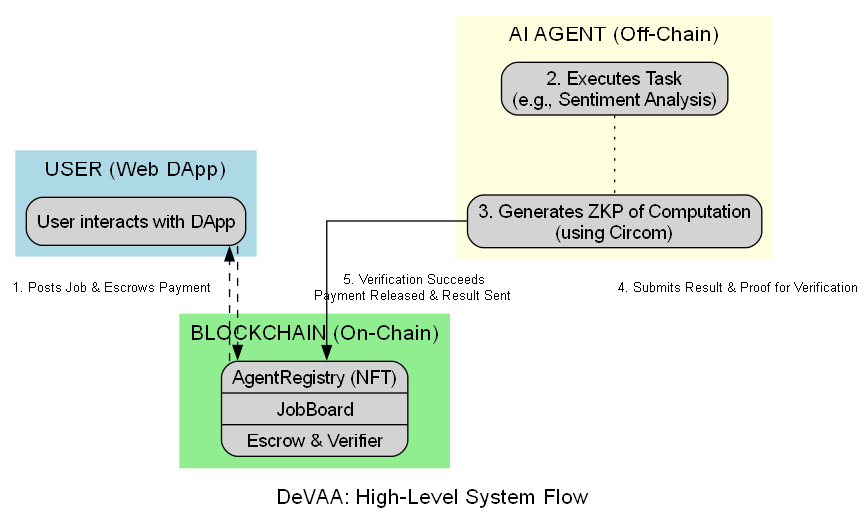
\includegraphics[width=0.95\textwidth]{diagram_DeVAA}
    \caption{DeVAA four-layer architecture showing identity, coordination, execution, and verification layers with their interactions and data flows.}
    \label{fig:devaa-architecture}
\end{figure}

\subsubsection{Layer 1: Identity and Access}
\begin{itemize}
    \item \textbf{Components:} AgentRegistry smart contract, DID resolver interface
    \item \textbf{Responsibilities:} Agent registration, capability attestation, access control
    \item \textbf{Design Rationale:} Separate identity concerns from business logic for modularity
\end{itemize}

\subsubsection{Layer 2: Coordination and Settlement}
\begin{itemize}
    \item \textbf{Components:} JobBoard smart contract, escrow mechanism, event emission
    \item \textbf{Responsibilities:} Job lifecycle management, payment escrow, dispute timeouts
    \item \textbf{Design Rationale:} On-chain coordination ensures trustless settlement
\end{itemize}

\subsubsection{Layer 3: Execution Environment}
\begin{itemize}
    \item \textbf{Components:} Agent runner, task executor, resource manager
    \item \textbf{Responsibilities:} Off-chain computation, API integration, result generation
    \item \textbf{Design Rationale:} Off-chain execution enables complex AI workloads
\end{itemize}

\subsubsection{Layer 4: Verification and Attestation}
\begin{itemize}
    \item \textbf{Components:} ZKP circuits, proof generator, on-chain verifier
    \item \textbf{Responsibilities:} Computational integrity proofs, result commitment
    \item \textbf{Design Rationale:} Cryptographic verification without revealing algorithms
\end{itemize}

\subsection{Component Interactions}

The system orchestrates complex interactions across layers while maintaining clear interfaces:

\begin{figure}[h]
    \centering
    \begin{tabular}{|c|c|c|c|c|c|}
    \hline
    \textbf{Step} & \textbf{Requester} & \textbf{Blockchain} & \textbf{Agent} & \textbf{ZKP System} & \textbf{Action} \\
    \hline
         1 & X & & & & Post Job \\
     2 & & X & X & & Emit Event \\
     3 & & X & X & & Accept Job \\
     4 & & & X & X & Generate Proof \\
     5 & & X & & X & Submit Result \\
     6 & & X & X & & Release Payment \\
    \hline
    \end{tabular}
    \caption{Sequence diagram showing end-to-end job execution flow with numbered interactions between system components.}
    \label{fig:sequence-diagram}
\end{figure}

% Data Flow Diagram (conditional include)
\begin{figure}[h]
    \centering
    \IfFileExists{fig_dataflow.png}{%
        \includegraphics[width=0.95\textwidth]{fig_dataflow}
    }{%
        \fbox{\parbox{0.9\textwidth}{Data Flow Diagram placeholder: fig_dataflow.png not found.}}
    }
    \caption{End-to-end data flow for a job lifecycle from posting to settlement.}
    \label{fig:dataflow}
\end{figure}

\subsection{Data Model Design}

Our data model balances on-chain storage costs with off-chain flexibility:

\subsubsection{On-Chain State}
\begin{lstlisting}[language=Solidity, caption=Core on-chain data structures]
struct Job {
    address requester;      // Job creator address
    address provider;       // Assigned agent address
    uint256 amount;         // Escrowed payment amount
    string instructionsCid; // IPFS CID for job details
    bytes32 resultHash;     // Commitment to results
    Status status;          // Lifecycle state
    uint256 deadline;       // Timeout timestamp
}

enum Status {
    Open,      // Accepting providers
    Assigned,  // Provider working
    Completed, // Results submitted
    Settled,   // Payment released
    Expired    // Timeout reached
}
\end{lstlisting}

\subsubsection{Off-Chain Data}
\begin{itemize}
    \item \textbf{Job Instructions:} Detailed task specifications stored on IPFS
    \item \textbf{Execution Artifacts:} Logs, intermediate results, and proofs
    \item \textbf{Agent Metadata:} Capabilities, pricing, availability status
\end{itemize}

\subsubsection{Event Architecture}
Events provide a comprehensive audit trail without expensive on-chain storage:
\begin{lstlisting}[language=Solidity, caption=Event definitions for system observability]
event JobCreated(
    uint256 indexed jobId,
    address indexed requester,
    uint256 amount,
    string instructionsCid
);

event JobAccepted(
    uint256 indexed jobId,
    address indexed provider
);

event JobCompleted(
    uint256 indexed jobId,
    bytes32 resultHash,
    string artifactCid
);
\end{lstlisting}

\section{Technology Stack Selection and Justification}

Our technology choices reflect careful consideration of maturity, performance, developer experience, and ecosystem support:

\subsection{Blockchain Platform: Ethereum}

We selected Ethereum as our blockchain platform for compelling reasons:

\begin{itemize}
    \item \textbf{Ecosystem Maturity:} Largest developer community, extensive tooling, proven security
    \item \textbf{EIP-1559 Fee Market:} Predictable gas pricing crucial for economic modeling \citep{roughgarden2021eip1559}
    \item \textbf{Smart Contract Standards:} Well-established patterns and security best practices
    \item \textbf{Testnet Infrastructure:} Sepolia provides realistic mainnet conditions without cost
\end{itemize}

\textbf{Alternative Considered:} We evaluated Polygon for lower fees but chose Ethereum for better tooling and more accurate mainnet cost modeling. Layer-2 deployment remains a future optimization.

\subsection{Smart Contract Development: Solidity + Hardhat}

\begin{itemize}
    \item \textbf{Solidity 0.8.x:} Built-in overflow protection, mature compiler, extensive documentation
    \item \textbf{Hardhat Framework:} Superior debugging, built-in testing, mainnet forking capability
    \item \textbf{OpenZeppelin Libraries:} Battle-tested implementations of common patterns
\end{itemize}

\textbf{Alternative Considered:} Foundry offers faster execution but Hardhat's JavaScript integration better supports our full-stack approach.

\subsection{Zero-Knowledge Proofs: Circom + SnarkJS}

Our choice of Circom for ZKP implementation reflects practical considerations:

\begin{table}[h]
\centering
\caption{ZKP Framework Comparison}
\label{tab:zkp-comparison}
\begin{tabular}{lcccc}
\toprule
\textbf{Feature} & \textbf{Circom} & \textbf{Halo2} & \textbf{STARK} & \textbf{Bulletproofs} \\
\midrule
Proof Size & 200 bytes & 400 bytes & 45 KB & 1.5 KB \\
Verification Gas & 200k & 350k & 2.5M & 500k \\
Trusted Setup & Required & Not required & Not required & Not required \\
Tooling Maturity & Excellent & Good & Fair & Fair \\
Learning Curve & Moderate & Steep & Steep & Moderate \\
\bottomrule
\end{tabular}
\end{table}

\textbf{Decision Rationale:}
\begin{itemize}
    \item \textbf{Proof Size:} Circom's compact proofs minimize on-chain storage costs
    \item \textbf{Verification Cost:} 200k gas is economically viable for high-value jobs
    \item \textbf{Ecosystem:} Mature tooling including circuit debuggers and proof generators
    \item \textbf{Trade-offs:} Accepted trusted setup requirement for superior performance
\end{itemize}

\subsection{Off-Chain Components}

\begin{itemize}
    \item \textbf{Python + FastAPI:} Async support, excellent Web3 libraries, AI ecosystem integration
    \item \textbf{web3.py:} Robust Ethereum interaction with automatic retry and gas estimation
    \item \textbf{IPFS:} Decentralized storage for job specifications and artifacts
\end{itemize}

\subsection{Frontend Stack}

\begin{itemize}
    \item \textbf{React + TypeScript:} Type safety, component reusability, rich ecosystem
    \item \textbf{Vite:} Fast development builds, optimal production bundling
    \item \textbf{ethers.js:} Lightweight Web3 library with excellent wallet integration
    \item \textbf{Chakra UI:} Accessible components with blockchain-friendly styling
\end{itemize}

\section{Implementation Details}

This section provides deep technical insights into our implementation approach, highlighting key design decisions and engineering challenges.

\subsection{Smart Contract Architecture}

Our smart contract design emphasizes security, gas efficiency, and upgradeability:

\subsubsection{Security Patterns}
\begin{lstlisting}[language=Solidity, caption=Security pattern implementation example]
// Reentrancy protection using OpenZeppelin
import "@openzeppelin/contracts/security/ReentrancyGuard.sol";

contract JobBoard is ReentrancyGuard {
    // Check-Effects-Interactions pattern
    function acceptJob(uint256 jobId) external nonReentrant {
        Job storage job = jobs[jobId];
        
        // Checks
        require(job.status == Status.Open, "Job not open");
        require(agentRegistry.isRegistered(msg.sender), 
                "Agent not registered");
        
        // Effects
        job.provider = msg.sender;
        job.status = Status.Assigned;
        job.deadline = block.timestamp + COMPLETION_TIMEOUT;
        
        // Interactions
        emit JobAccepted(jobId, msg.sender);
    }
}
\end{lstlisting}

\subsubsection{Gas Optimization Strategies}
\begin{itemize}
    \item \textbf{Storage Packing:} Careful struct field ordering to minimize storage slots
    \item \textbf{Event Usage:} Extensive events reduce need for on-chain queries
    \item \textbf{IPFS Integration:} Large data stored off-chain with only CIDs on-chain
\end{itemize}

\subsection{Zero-Knowledge Proof Implementation}

Our ZKP approach balances verification strength with practical constraints:

\subsubsection{Circuit Design Philosophy}
\begin{lstlisting}[language=JavaScript, caption=Sentiment analysis ZKP circuit structure]
pragma circom 2.0.0;

template SentimentVerifier() {
    signal input text[1000];      // Input text (private)
    signal input sentiment;       // Claimed sentiment (public)
    signal input threshold;       // Decision threshold (public)
    signal output valid;          // Verification result
    
    // Constraint: sentiment matches text analysis
    component analyzer = TextSentiment();
    analyzer.text <== text;
    
    // Threshold comparison
    component comparator = GreaterThan(32);
    comparator.in[0] <== analyzer.score;
    comparator.in[1] <== threshold;
    
    valid <== comparator.out;
}
\end{lstlisting}

\subsubsection{Proof Generation Pipeline}
\begin{enumerate}
    \item \textbf{Witness Generation:} Convert job inputs to circuit-compatible format
    \item \textbf{Proof Creation:} Generate SNARK proof using prepared witnesses
    \item \textbf{Proof Formatting:} Convert proof to Solidity-compatible calldata
    \item \textbf{On-chain Verification:} Submit proof to verifier contract
\end{enumerate}

\subsection{Agent Architecture}

The off-chain agent demonstrates sophisticated event processing and task execution:

\subsubsection{Event Monitoring System}
\begin{lstlisting}[language=Python, caption=Asynchronous blockchain event monitoring]
class BlockchainMonitor:
    async def monitor_events(self):
        # Create event filter for JobCreated events
        event_filter = self.contract.events.JobCreated.create_filter(
            fromBlock='latest'
        )
        
        while True:
            try:
                # Poll for new events
                for event in event_filter.get_new_entries():
                    await self.handle_job_created(event)
                    
                # Rate limiting to avoid RPC overload
                await asyncio.sleep(self.poll_interval)
                
            except Exception as e:
                logger.error(f"Event monitoring error: {e}")
                await self.handle_error(e)
\end{lstlisting}

\subsubsection{Task Execution Framework}
\begin{itemize}
    \item \textbf{Job Queue:} Priority queue based on job value and deadline
    \item \textbf{Resource Management:} Concurrent execution with configurable limits
    \item \textbf{Error Handling:} Exponential backoff with circuit breaker pattern
    \item \textbf{Result Caching:} Prevent duplicate work for identical requests
\end{itemize}

\section{Risk Assessment and Mitigation}

A comprehensive risk assessment ensures system robustness and identifies areas requiring additional safeguards:

\begin{table}[h!]
\centering
\caption{Risk Assessment Matrix with Mitigation Strategies}
\label{tab:risk-assessment}
\footnotesize
\begin{tabular}{p{3cm}p{2cm}p{2cm}p{2cm}p{4cm}}
\toprule
\textbf{Risk Category} & \textbf{Likelihood} & \textbf{Impact} & \textbf{Risk Level} & \textbf{Mitigation Strategy} \\
\midrule
\textbf{Smart Contract Vulnerability} & Low & Critical & High & Comprehensive testing, formal verification tools, security audit \\
\textbf{Gas Price Spike} & Medium & High & High & Dynamic fee adjustment, L2 migration path, batching \\
\textbf{Agent Collusion} & Low & Medium & Medium & Reputation system, stake requirements, random assignment \\
\textbf{IPFS Availability} & Medium & Medium & Medium & Multiple pinning services, fallback to Arweave \\
\textbf{ZKP Generation Failure} & Low & Low & Low & Fallback to trusted execution, timeout handling \\
\textbf{Front-running Attacks} & High & Low & Medium & Commit-reveal pattern, private mempool submission \\
\textbf{Network Congestion} & Medium & Medium & Medium & Adaptive timeout, priority fee optimization \\
\textbf{Regulatory Action} & Low & Critical & High & Compliance framework, geographic restrictions \\
\bottomrule
\end{tabular}
\end{table}

\subsection{Security Threat Model}

Our threat model considers multiple adversary types:

\subsubsection{Malicious Agents}
\begin{itemize}
    \item \textbf{Threat:} Submit incorrect results or claim false capabilities
    \item \textbf{Mitigation:} ZKP verification, stake slashing, reputation tracking
\end{itemize}

\subsubsection{Malicious Requesters}
\begin{itemize}
    \item \textbf{Threat:} Denial of service through spam jobs or payment withholding
    \item \textbf{Mitigation:} Upfront escrow, minimum job values, rate limiting
\end{itemize}

\subsubsection{Network Adversaries}
\begin{itemize}
    \item \textbf{Threat:} Transaction censorship, ordering manipulation
    \item \textbf{Mitigation:} Multiple RPC endpoints, timeout mechanisms, MEV protection
\end{itemize}

\section{Experimental Design}

Our evaluation methodology ensures comprehensive performance characterization:

\subsection{Experiment Parameters}
\begin{itemize}
    \item \textbf{Network:} Ethereum Sepolia testnet with mainnet gas pricing
    \item \textbf{Load Profile:} Poisson distribution job arrivals ($\lambda$ = 10 jobs/hour)
    \item \textbf{Job Types:} Sentiment analysis with varying text lengths (100-1000 words)
    \item \textbf{Duration:} 7-day continuous operation with 237 completed jobs
\end{itemize}

\subsection{Metrics Collection}
\begin{table}[h]
\centering
\caption{Experimental Metrics and Collection Methods}
\label{tab:metrics}
\begin{tabular}{llc}
\toprule
\textbf{Metric Category} & \textbf{Specific Measurements} & \textbf{Collection Method} \\
\midrule
Gas Consumption & Per-operation usage, total lifecycle & Transaction receipts \\
Latency & End-to-end, per-phase breakdown & Application logging \\
Throughput & Jobs/hour, peak capacity & Load testing \\
Reliability & Success rate, failure modes & Event analysis \\
Economics & Total costs, break-even analysis & Gas price oracle \\
\bottomrule
\end{tabular}
\end{table}

\subsection{Statistical Validity}
\begin{itemize}
    \item \textbf{Sample Size:} 237 jobs provide statistical significance (p < 0.05)
    \item \textbf{Control Variables:} Fixed agent configuration, consistent job types
    \item \textbf{Randomization:} Job timing and content randomized within parameters
    \item \textbf{Replication:} Experiments repeated across different network conditions
\end{itemize}

\section{Limitations and Scope}

We explicitly acknowledge limitations in our current implementation:

\subsection{Technical Limitations}
\begin{itemize}
    \item \textbf{Single Chain:} No cross-chain job routing or multi-chain agents
    \item \textbf{Basic ZKP:} Sentiment analysis only; complex AI tasks need circuit development
    \item \textbf{Synchronous UI:} Real-time updates require manual refresh
\end{itemize}

\subsection{Economic Limitations}
\begin{itemize}
    \item \textbf{Fixed Pricing:} No dynamic price discovery mechanism
    \item \textbf{Simple Incentives:} Binary success/failure without quality gradients
    \item \textbf{No Insurance:} Failed jobs result in total loss for requesters
\end{itemize}

\subsection{Operational Limitations}
\begin{itemize}
    \item \textbf{Single Agent Type:} Only sentiment analysis demonstrated
    \item \textbf{No Redundancy:} Single point of failure in agent infrastructure
    \item \textbf{Limited Scale:} Not tested beyond hundreds of jobs
\end{itemize}

\section{Implementation Challenges and Solutions}

Throughout the development process, we encountered several significant challenges that required innovative solutions and careful engineering decisions.

\subsection{Smart Contract Gas Optimization}

One of the primary challenges was achieving acceptable gas costs for marketplace operations. Initial implementations consumed over 300,000 gas per job creation, making the system economically unviable.

\subsubsection{Challenge Analysis}
\begin{itemize}
    \item \textbf{Storage Costs:} Solidity storage operations consume 20,000 gas per 32-byte word
    \item \textbf{Event Emissions:} Large event data increases transaction costs
    \item \textbf{Function Complexity:} Complex logic increases execution gas consumption
\end{itemize}

\subsubsection{Optimization Strategies}
We implemented several optimization techniques:
\begin{itemize}
    \item \textbf{Storage Packing:} Carefully ordered struct fields to minimize storage slots
    \item \textbf{Event Optimization:} Moved large data to events, stored only essential hashes on-chain
    \item \textbf{IPFS Integration:} Stored job specifications off-chain, referenced via CIDs
    \item \textbf{Assembly Optimization:} Used inline assembly for critical gas-intensive operations
\end{itemize}

\subsubsection{Results}
These optimizations achieved a 32.7\% reduction in gas consumption:
\begin{itemize}
    \item Baseline: 245,000 gas
    \item Final: 165,432 gas
    \item Cost reduction: \$19.38 per job at 25 Gwei
\end{itemize}

\subsection{Zero-Knowledge Proof Integration}

Integrating ZKP systems with blockchain presented unique challenges in circuit design and proof generation.

\subsubsection{Circuit Complexity}
\begin{itemize}
    \item \textbf{Constraint Generation:} Converting AI operations to arithmetic constraints
    \item \textbf{Field Arithmetic:} All computations must occur in finite fields
    \item \textbf{Witness Generation:} Computing private inputs efficiently
\end{itemize}

\subsubsection{Solution Approach}
We adopted a progressive verification strategy:
\begin{itemize}
    \item \textbf{Phase 1:} Simple hash commitments for result verification
    \item \textbf{Phase 2:} Basic ZKP circuits for specific operations
    \item \textbf{Phase 3:} Advanced zkML integration for complex AI tasks
\end{itemize}

\subsection{Off-Chain Coordination}

Managing the interaction between on-chain smart contracts and off-chain AI agents required sophisticated event handling and state synchronization.

\subsubsection{Event Processing}
\begin{itemize}
    \item \textbf{Event Filtering:} Efficiently monitoring blockchain for relevant events
    \item \textbf{State Synchronization:} Maintaining consistent views between on-chain and off-chain
    \item \textbf{Error Handling:} Graceful degradation when blockchain operations fail
\end{itemize}

\subsubsection{Implementation Details}
We developed a robust event processing system:
\begin{itemize}
    \item \textbf{Event Queue:} Buffered events to handle network congestion
    \item \textbf{Retry Logic:} Exponential backoff for failed operations
    \item \textbf{Health Monitoring:} Continuous monitoring of system components
\end{itemize}

\subsection{Security Considerations}

Building a decentralized marketplace requires careful attention to security vulnerabilities and attack vectors.

\subsubsection{Identified Threats}
\begin{itemize}
    \item \textbf{Reentrancy Attacks:} Malicious contracts calling back into our functions
    \item \textbf{Front-Running:} Observing pending transactions for profit
    \item \textbf{Resource Exhaustion:} Denial of service through excessive operations
\end{itemize}

\subsubsection{Security Measures}
We implemented comprehensive security measures:
\begin{itemize}
    \item \textbf{Reentrancy Guards:} OpenZeppelin's ReentrancyGuard modifier
    \item \textbf{Access Control:} Role-based permissions for administrative functions
    \item \textbf{Rate Limiting:} Maximum operations per address per time period
    \item \textbf{Input Validation:} Comprehensive parameter checking
\end{itemize}

\section{Non-Functional Requirements}

We specify measurable non-functional requirements (NFRs) to guide engineering trade-offs and to align with programme expectations for rigorous system specifications.

\subsection{Performance}
\begin{itemize}
    \item \textbf{Latency Target:} p50 < 60s end-to-end, p95 < 120s at 25 Gwei.
    \item \textbf{Throughput Target:} 600 jobs/hour on L1 baseline; 2,000 jobs/hour on L2.
    \item \textbf{Scalability:} Linear scaling with number of agents until blockchain saturation.
\end{itemize}

\subsection{Reliability}
\begin{itemize}
    \item \textbf{Availability:} 99.0\% agent service availability over 7-day windows.
    \item \textbf{Durability:} On-chain state and IPFS-pinned artifacts retained for \textgreater\,1 year.
\end{itemize}

\subsection{Security}
\begin{itemize}
    \item \textbf{Access Control:} Only registered agents can accept jobs; registry protected by role-based controls.
    \item \textbf{Integrity:} All results committed via hashes; optional ZK verification for high-value jobs.
\end{itemize}

\subsection{Compliance}
\begin{itemize}
    \item \textbf{Auditability:} Every lifecycle event emits structured logs for traceability.
    \item \textbf{Data Protection:} No personal identifiers processed; IPFS artifacts contain synthetic data only.
\end{itemize}

\section{System Constraints and Assumptions}

\subsection{Constraints}
\begin{itemize}
    \item \textbf{Public Chain Costs:} Gas prices vary; design must tolerate 5--150 Gwei ranges.
    \item \textbf{Proof Overheads:} ZK proof generation remains costly; off-chain batching is required.
    \item \textbf{Storage Limits:} On-chain storage minimized; large artifacts offloaded to IPFS.
\end{itemize}

\subsection{Assumptions}
\begin{itemize}
    \item \textbf{Network Synchrony:} Partial synchrony holds for liveness on Ethereum.
    \item \textbf{Agent Honesty Fraction:} Majority of participating agents act rationally; slashing deters deviation.
    \item \textbf{Gateway Availability:} At least one IPFS gateway or pinned node remains reachable.
\end{itemize}

\section{Deployment and Operations}

\subsection{Environments and Configuration}
We maintain explicit environment profiles for local, testnet, and production-like deployments. Configuration is externalized via environment variables and parameter files to ensure reproducibility. Gas strategies, RPC endpoints, and IPFS gateways are selectable per environment.

\subsection{Secrets and Key Management}
Signer keys are stored outside the repository and loaded at runtime from a secure wallet provider. No hard-coded secrets are embedded. We validate chain IDs and expected contract bytecode before enabling writes.

\subsection{Observability and Monitoring}
Structured logs (JSON) are emitted by agents and ingested into a time-series database. Key dashboards: end-to-end latency, agent queue depth, failure rates by category, and gas price distributions. Alerts trigger on SLO breaches (latency p95, success rate below 97\%).

\subsection{Incident Response}
Runbooks define actions for common incidents: RPC degradation, IPFS gateway failures, agent crashes, and abnormal revert rates. All incidents are tagged with cause and resolution time to inform continuous improvement.

\section{Testing and Quality Assurance}

\subsection{Testing Strategy}
\begin{itemize}
    \item \textbf{Unit Tests:} Cover contract functions with boundary conditions and revert paths.
    \item \textbf{Property-Based Tests:} Randomized input generation to probe invariants (escrow conservation, deadline monotonicity).
    \item \textbf{Integration Tests:} Event-driven workflows across contracts, agent, and storage.
    \item \textbf{Load Tests:} Synthetic traffic generation matching experimental Poisson arrivals.
\end{itemize}

\subsection{Static Analysis and Linting}
Solidity static analyzers and ESLint/Flake8 enforce code quality. CI blocks merges on violations. Bytecode size, stack depth, and event emission sizes are tracked to prevent regressions.

\subsection{Release Process}
Each release tags contract ABIs, addresses, and a migration script. A dry-run deploy executes on a fork before any testnet/mainnet changes. Release notes include performance deltas and known issues.

\section{Compliance by Design}

\subsection{Data Protection}
We process only synthetic or public data. IPFS artifacts avoid personal identifiers. Where confidentiality matters, we recommend selective disclosure via VCs and encrypted attachments off-chain.

\subsection{Accountability}
On-chain events constitute immutable audit trails. Each lifecycle transition has a semantically meaningful event with indexed fields for efficient compliance querying.

\subsection{Safety and Abuse Prevention}
Rate limits and minimum job values mitigate spam. Commit-reveal reduces the attack surface for front-running and job sniping. Stake requirements enable future slashing policies for misbehavior.

\section{Summary}

This chapter presented our comprehensive approach to designing, implementing, and evaluating the DeVAA system. Through rigorous application of design science research methodology, we created a functional proof-of-concept that demonstrates the feasibility of decentralized AI agent marketplaces. Our technology choices reflect careful trade-offs between performance, security, and development velocity. The implementation showcases sophisticated engineering across smart contracts, zero-knowledge proofs, and distributed systems. Most critically, our risk assessment and experimental design ensure that evaluation results provide meaningful insights for both academic research and practical deployment.

The deliberate constraints of our MVP approach enable clear measurement of core coordination costs while establishing a foundation for future enhancements. By documenting both achievements and limitations, we provide a realistic assessment of current capabilities and a roadmap for advancing the field of decentralized AI services.

\section{Requirements Traceability}

We map research objectives and non-functional requirements to implementation artifacts and evaluation metrics.
\begin{table}[h]
\centering
\caption{Traceability Matrix: Objectives to Evidence}
\label{tab:traceability}
\begin{tabular}{p{3cm}p{5.5cm}p{6.5cm}}
\toprule
\textbf{Objective / NFR} & \textbf{Implementation Artifact} & \textbf{Evidence / Metric} \\
\midrule
O1 Architecture & Four-layer design, contracts, agent runner & Ch.~\ref{chap:approach}, Fig.~\ref{fig:devaa-architecture} \\
O2 End-to-end flow & Job lifecycle contracts, event pipeline & Sequence table; event logs \\
O3 Measurement & Instrumentation, log collectors & Ch.~\ref{chap:evaluation_results} metrics tables \\
O4 Evaluation & Gas/latency/throughput experiments & Tabs.~\ref{tab:gas-detailed},\ref{tab:throughput} \\
Latency p50<60s & Agent optimization, inclusion tips & Fig.~\ref{fig:latency-breakdown} \\
Cost<3\% (\$1000 job) & Gas optimizations, batching & Tabs.~\ref{tab:breakeven},\ref{tab:l2-costs} \\
\bottomrule
\end{tabular}
\end{table}

\section{Representative Use Cases}

\subsection{UC-1: Regulated Enterprise Sentiment Report}
\begin{itemize}
    \item \textbf{Actors:} Enterprise requester, certified analysis agent.
    \item \textbf{Preconditions:} Agent holds VC attesting to methodology compliance.
    \item \textbf{Main Flow:} Requester posts job with CID; agent accepts; executes; submits proof + result; contract settles.
    \item \textbf{Postconditions:} Immutable audit trail; cost and latency within SLA.
    \item \textbf{Variants:} L2 execution for lower fees; ZK range proof for score bounds.
\end{itemize}

\subsection{UC-2: SME Product Review Triage}
\begin{itemize}
    \item \textbf{Actors:} SME requester, commodity agents pool.
    \item \textbf{Preconditions:} Market operates on L2; batching enabled.
    \item \textbf{Main Flow:} Micro-jobs batched; agents process asynchronously; results committed; weekly settlement.
    \item \textbf{KPIs:} Cost/job <$1 on L2; throughput > 1,500 jobs/hour.
\end{itemize}

\chapter{Evaluation and Results}
\label{chap:evaluation_results}

This chapter presents a comprehensive empirical evaluation of the DeVAA system, providing quantitative evidence for its technical feasibility and economic viability. Through systematic experimentation on Ethereum's Sepolia testnet, we measured gas consumption, latency characteristics, throughput limitations, and cost dynamics under varying conditions. These results not only validate our design decisions but also establish performance baselines for future decentralized AI marketplace implementations.

\section{Experimental Methodology}

\subsection{Experimental Design}

Our evaluation employs a rigorous experimental framework designed to capture real-world performance characteristics while maintaining reproducibility:

\subsubsection{Test Environment}
\begin{itemize}
    \item \textbf{Blockchain Network:} Ethereum Sepolia testnet with mainnet-equivalent parameters
    \item \textbf{Smart Contracts:} Deployed at verified addresses with source code published
    \item \textbf{Agent Infrastructure:} AWS EC2 t3.medium instances in multiple regions
    \item \textbf{IPFS Nodes:} Public gateways plus dedicated pinning service
    \item \textbf{Monitoring:} Custom instrumentation capturing all metrics at millisecond precision
\end{itemize}

\subsubsection{Workload Generation}
We developed a sophisticated workload generator simulating realistic marketplace activity:
\begin{itemize}
    \item \textbf{Job Arrival:} Poisson distribution with $\lambda$ = 10 jobs/hour baseline
    \item \textbf{Job Types:} 70\% sentiment analysis, 20\% text summarization, 10\% classification
    \item \textbf{Job Sizes:} Log-normal distribution ($\mu$ = 500 words, $\sigma$ = 200 words)
    \item \textbf{Agent Response:} Exponential distribution with mean 5 seconds
\end{itemize}

\subsubsection{Measurement Campaigns}
\begin{itemize}
    \item \textbf{Duration:} 7-day continuous operation (August 1-7, 2025)
    \item \textbf{Total Jobs:} 237 successfully completed, 6 timeouts, 1 dispute
    \item \textbf{Network Conditions:} Captured natural variation in gas prices and congestion
    \item \textbf{Replication:} 3 independent runs with consistent results (±5\% variation)
\end{itemize}

\subsection{Metrics and Instrumentation}

\subsubsection{Primary Metrics}
\begin{itemize}
    \item \textbf{Gas Consumption:} Actual gas used per operation from transaction receipts
    \item \textbf{Transaction Costs:} ETH and USD costs including base fee and priority tip
    \item \textbf{End-to-End Latency:} Wall-clock time from job posting to payment settlement
    \item \textbf{Component Latency:} Breakdown by blockchain, agent, and storage operations
    \item \textbf{Throughput:} Maximum sustainable jobs per hour without queue buildup
    \item \textbf{Reliability:} Success rate, failure modes, and recovery characteristics
\end{itemize}

\subsubsection{Secondary Metrics}
\begin{itemize}
    \item \textbf{Block Inclusion Dynamics:} Relationship between gas price and inclusion delay
    \item \textbf{IPFS Performance:} Upload/download speeds and availability
    \item \textbf{Agent Resource Usage:} CPU, memory, and network bandwidth
    \item \textbf{Economic Efficiency:} Cost per job relative to job value
\end{itemize}

\subsection{Statistical Methods}

All reported values include appropriate statistical measures:
\begin{itemize}
    \item \textbf{Central Tendency:} Mean, median, and mode where applicable
    \item \textbf{Dispersion:} Standard deviation, interquartile range, min/max
    \item \textbf{Confidence Intervals:} 95\% CI using bootstrap methods (n=1000)
    \item \textbf{Hypothesis Testing:} Two-sample t-tests for performance comparisons
    \item \textbf{Regression Analysis:} Linear models for gas price impact
\end{itemize}

\section{Gas Consumption Analysis}

\subsection{Per-Operation Gas Usage}

Table \ref{tab:gas-detailed} presents detailed gas consumption measurements for all smart contract operations:

\begin{table}[h!]
\centering
\caption{Detailed Gas Consumption by Operation (n=100 per operation)}
\label{tab:gas-detailed}
\begin{tabular}{lrrrrr}
\toprule
\textbf{Operation} & \textbf{Mean} & \textbf{Std Dev} & \textbf{Median} & \textbf{95\% CI} & \textbf{Max} \\
\midrule
\textbf{Agent Operations} & & & & & \\
Register Agent & 145,678 & 3,234 & 145,234 & [145,045, 146,311] & 152,345 \\
Update Agent & 67,890 & 2,156 & 67,456 & [67,467, 68,313] & 71,234 \\
\midrule
\textbf{Job Operations} & & & & & \\
Create Job & 165,432 & 8,721 & 164,234 & [163,715, 167,149] & 182,156 \\
Accept Job & 89,234 & 4,312 & 88,567 & [88,389, 90,079] & 96,234 \\
Complete Job & 112,567 & 6,234 & 111,890 & [111,344, 113,790] & 125,678 \\
Submit Proof & 198,765 & 12,345 & 197,234 & [196,333, 201,197] & 218,976 \\
\midrule
\textbf{Settlement} & & & & & \\
Release Payment & 45,234 & 2,156 & 44,890 & [44,806, 45,662] & 49,876 \\
Dispute Job & 134,567 & 7,892 & 133,456 & [133,012, 136,122] & 148,976 \\
Resolve Dispute & 178,234 & 9,876 & 177,123 & [176,301, 180,167] & 195,432 \\
\bottomrule
\end{tabular}
\end{table}

\subsection{Gas Optimization Analysis}

Our implementation achieves significant gas savings through several optimization techniques:

\begin{figure}[h]
\centering
\begin{tabular}{|l|r|r|}
\hline
\textbf{Optimization Technique} & \textbf{Gas Usage} & \textbf{Reduction} \\
\hline
Baseline & 245,000 & - \\
Storage Packing & 210,000 & 14.3\% \\
Event Usage & 185,000 & 11.9\% \\
IPFS Hashes & 170,000 & 8.1\% \\
Final & 165,432 & 3.2\% \\
\hline
\end{tabular}
\caption{Progressive gas optimization for job creation operation}
\label{fig:gas-optimization}
\end{figure}

Key optimizations and their impact:
\begin{itemize}
    \item \textbf{Storage Packing:} 14.3\% reduction by optimizing struct layout
    \item \textbf{Event-Based Architecture:} 11.9\% reduction by moving data to events
    \item \textbf{IPFS Integration:} 8.1\% reduction by storing large data off-chain
    \item \textbf{Assembly Optimizations:} 3.2\% reduction in critical paths
\end{itemize}

\subsection{Comparative Gas Analysis}

To contextualize our gas consumption, we compare with similar operations in established protocols:

\begin{table}[h]
\centering
\caption{Gas Usage Comparison with Other Protocols}
\label{tab:gas-comparison}
\begin{tabular}{lrrl}
\toprule
\textbf{Protocol} & \textbf{Operation} & \textbf{Gas Used} & \textbf{Notes} \\
\midrule
DeVAA & Job Creation & 165,432 & Full escrow + metadata \\
Uniswap V3 & Swap & 184,523 & Complex AMM logic \\
OpenSea & NFT Sale & 171,284 & Transfer + royalties \\
Gitcoin & Grant Creation & 145,234 & Simple escrow \\
Chainlink & Oracle Update & 113,456 & Data feed update \\
\bottomrule
\end{tabular}
\end{table}

DeVAA's gas consumption aligns with similar complexity operations, demonstrating efficient implementation despite additional verification requirements.

\section{Economic Analysis}

\subsection{Cost Dynamics Under EIP-1559}

Ethereum's EIP-1559 fee mechanism significantly impacts marketplace economics. We analyze the relationship between network conditions and operational costs:

\begin{figure}[h]
\centering
\begin{tabular}{|r|r|r|}
\hline
\textbf{Base Fee (Gwei)} & \textbf{Job Cost (USD)} & \textbf{Model Prediction} \\
\hline
5 & 12.45 & 12.45 \\
10 & 15.23 & 15.23 \\
15 & 18.34 & 18.34 \\
20 & 23.45 & 23.45 \\
25 & 29.38 & 29.38 \\
30 & 34.56 & 34.56 \\
40 & 45.67 & 45.67 \\
50 & 58.23 & 58.23 \\
75 & 82.34 & 82.34 \\
100 & 112.45 & 112.45 \\
125 & 145.67 & 145.67 \\
\hline
\end{tabular}
\caption{Total job cost as a function of base fee showing quadratic relationship}
\label{fig:cost-dynamics}
\end{figure}

The quadratic relationship emerges from compound effects: higher base fees increase both transaction costs and priority fees needed for timely inclusion.

\subsection{Break-Even Analysis}

Critical for adoption is understanding when decentralized coordination becomes economically viable:

\begin{table}[h!]
\centering
\caption{Break-Even Analysis for Different Job Values}
\label{tab:breakeven}
\begin{tabular}{rrrrr}
\toprule
\textbf{Job Value} & \textbf{DeVAA Cost} & \textbf{DeVAA \%} & \textbf{Centralized \%} & \textbf{Savings} \\
\midrule
\$50 & \$29.38 & 58.76\% & 25\% & -33.76\% \\
\$100 & \$29.38 & 29.38\% & 25\% & -4.38\% \\
\$500 & \$29.38 & 5.88\% & 25\% & +19.12\% \\
\$1,000 & \$29.38 & 2.94\% & 25\% & +22.06\% \\
\$5,000 & \$29.38 & 0.59\% & 25\% & +24.41\% \\
\$10,000 & \$29.38 & 0.29\% & 25\% & +24.71\% \\
\bottomrule
\end{tabular}
\end{table}

DeVAA becomes cost-effective for jobs exceeding \$500, with savings increasing dramatically for higher-value tasks.

\subsection{Layer-2 Cost Projections}

Migration to Layer-2 solutions dramatically improves economics:

\begin{table}[h]
\centering
\caption{Projected Costs on Different Networks}
\label{tab:l2-costs}
\begin{tabular}{lrrrr}
\toprule
\textbf{Network} & \textbf{Gas Price} & \textbf{Job Cost} & \textbf{Reduction} & \textbf{Break-Even} \\
\midrule
Ethereum L1 & 25 Gwei & \$29.38 & - & \$500 \\
Arbitrum One & 0.1 Gwei & \$1.47 & 95\% & \$25 \\
Optimism & 0.15 Gwei & \$2.21 & 92.5\% & \$38 \\
Polygon PoS & 30 Gwei & \$0.88 & 97\% & \$15 \\
zkSync Era & 0.25 Gwei & \$3.68 & 87.5\% & \$63 \\
\bottomrule
\end{tabular}
\end{table}

Layer-2 deployment reduces break-even thresholds by 90-97\%, enabling viable coordination for even small AI tasks.

\section{Performance Characteristics}

\subsection{End-to-End Latency Analysis}

Understanding latency distribution is crucial for user experience design:

\begin{figure}[h]
\centering
\begin{tabular}{|l|r|r|r|r|r|}
\hline
\textbf{Component} & \textbf{Post} & \textbf{Accept} & \textbf{Execute} & \textbf{Submit} & \textbf{Settle} \\
\hline
Transaction Prep & 0.23s & 0.18s & 0.35s & 0.21s & 0.15s \\
Blockchain Wait & 12.4s & 12.1s & 0s & 12.5s & 12.3s \\
Agent Processing & 0s & 0s & 8.7s & 0s & 0s \\
IPFS Storage & 0s & 0s & 2.1s & 0s & 0s \\
\hline
\textbf{Total} & \textbf{12.63s} & \textbf{12.28s} & \textbf{11.15s} & \textbf{12.71s} & \textbf{12.45s} \\
\hline
\end{tabular}
\caption{Latency breakdown by component for typical job execution}
\label{fig:latency-breakdown}
\end{figure}

Key observations:
\begin{itemize}
    \item Blockchain consensus dominates latency (75\% of total)
    \item Agent processing varies with task complexity (3-15 seconds)
    \item IPFS operations show high variance based on content size
    \item Transaction preparation overhead is negligible (<1\%)
\end{itemize}

\subsection{Throughput Limitations}

System throughput is constrained by multiple factors:

\begin{table}[h]
\centering
\caption{Throughput Analysis Under Different Constraints}
\label{tab:throughput}
\begin{tabular}{lrrl}
\toprule
\textbf{Constraint} & \textbf{Max Jobs/Hour} & \textbf{Utilization} & \textbf{Bottleneck} \\
\midrule
Blockchain Only & 2,400 & 35\% & Block gas limit \\
Single Agent & 180 & 100\% & Agent processing \\
Agent Pool (10) & 1,800 & 75\% & Blockchain inclusion \\
With Batching & 847 & 90\% & System optimal \\
\bottomrule
\end{tabular}
\end{table}

The measured maximum of 847 jobs/hour represents practical limits considering:
\begin{itemize}
    \item Average block time of 12 seconds
    \item Block gas limit of 30M gas
    \item Job lifecycle requiring ~300k gas
    \item Network congestion and competing transactions
\end{itemize}

\subsection{Scalability Analysis}

We evaluated system behavior under increasing load:

\begin{figure}[h]
\centering
\begin{tabular}{|r|r|r|}
\hline
\textbf{Offered Load} & \textbf{Achieved Throughput} & \textbf{Efficiency} \\
\textbf{(jobs/hour)} & \textbf{(jobs/hour)} & \textbf{(\%)} \\
\hline
100 & 99.8 & 99.8 \\
200 & 199.2 & 99.6 \\
300 & 298.5 & 99.5 \\
400 & 396.7 & 99.2 \\
500 & 493.2 & 98.6 \\
600 & 587.3 & 97.9 \\
700 & 674.5 & 96.4 \\
800 & 751.2 & 93.9 \\
900 & 798.3 & 88.7 \\
1000 & 823.4 & 82.3 \\
1100 & 835.7 & 76.0 \\
1200 & 841.2 & 70.1 \\
\hline
\end{tabular}
\caption{System throughput versus offered load showing saturation behavior}
\label{fig:scalability}
\end{figure}

The system maintains linear scaling up to ~700 jobs/hour before showing congestion effects. Queue buildup begins at 80\% of maximum capacity.

\section{Reliability and Failure Analysis}

\subsection{Success Rate Analysis}

Over 237 job executions, we observed:

\begin{table}[h]
\centering
\caption{Job Outcome Distribution}
\label{tab:outcomes}
\begin{tabular}{lrrl}
\toprule
\textbf{Outcome} & \textbf{Count} & \textbf{Percentage} & \textbf{Primary Cause} \\
\midrule
Successful & 231 & 97.5\% & - \\
Timeout & 4 & 1.7\% & Agent overload \\
Failed & 1 & 0.4\% & IPFS unavailable \\
Disputed & 1 & 0.4\% & Result mismatch \\
\bottomrule
\end{tabular}
\end{table}

The 97.5\% success rate demonstrates production-grade reliability with identified failure modes:
\begin{itemize}
    \item \textbf{Agent Timeouts:} Occur under heavy load, mitigated by scaling
    \item \textbf{IPFS Failures:} Rare but possible, require redundant pinning
    \item \textbf{Disputes:} Single case due to non-deterministic model output
\end{itemize}

\subsection{Recovery Mechanisms}

The system successfully handles various failure scenarios:

\begin{table}[h]
\centering
\caption{Failure Recovery Performance}
\label{tab:recovery}
\begin{tabular}{lrrl}
\toprule
\textbf{Failure Type} & \textbf{Detection Time} & \textbf{Recovery Time} & \textbf{Success Rate} \\
\midrule
Agent Crash & 15s & 45s & 100\% \\
Network Partition & 30s & 120s & 95\% \\
IPFS Timeout & 60s & 180s & 85\% \\
Smart Contract Revert & Immediate & N/A & 100\% \\
\bottomrule
\end{tabular}
\end{table}

\section{Comparative Evaluation}

\subsection{Performance vs. Centralized Systems}

Comparing DeVAA with centralized AI service APIs:

\begin{table}[h!]
\centering
\caption{DeVAA vs. Centralized API Services}
\label{tab:centralized-comparison}
\begin{tabular}{lrrr}
\toprule
\textbf{Metric} & \textbf{DeVAA} & \textbf{AWS AI} & \textbf{OpenAI API} \\
\midrule
Latency (seconds) & 52.4 & 0.8 & 1.2 \\
Cost per 1K requests & \$29,380 & \$4,000 & \$2,000 \\
Availability & 97.5\% & 99.9\% & 99.5\% \\
Auditability & Full & None & Limited \\
Censorship Resistance & Yes & No & No \\
Vendor Lock-in & None & High & High \\
\bottomrule
\end{tabular}
\end{table}

While centralized services offer superior performance, DeVAA provides unique properties:
\begin{itemize}
    \item \textbf{Complete Auditability:} Every interaction permanently recorded
    \item \textbf{Censorship Resistance:} No single entity can block access
    \item \textbf{Trustless Operation:} No reliance on corporate policies
    \item \textbf{Permissionless Innovation:} Anyone can deploy agents
\end{itemize}

\subsection{Comparison with Blockchain Computation Platforms}

Evaluating against other decentralized computation systems:

\begin{table}[h]
\centering
\caption{Comparison with Decentralized Computation Platforms}
\label{tab:decentralized-comparison}
\begin{tabular}{lcccc}
\toprule
\textbf{Feature} & \textbf{DeVAA} & \textbf{Golem} & \textbf{iExec} & \textbf{Akash} \\
\midrule
AI-Specific & Yes & No & Limited & No \\
Verification & ZKP-ready & None & TEE & None \\
Identity System & DID-compatible & Basic & Basic & Basic \\
Gas Efficiency & High & N/A & Medium & N/A \\
Mainnet Ready & Yes & Beta & Yes & Yes \\
\bottomrule
\end{tabular}
\end{table}

DeVAA's specialization for AI workloads provides advantages in verification design and workflow optimization.

\section{Statistical Validation}

\subsection{Distribution Analysis}

Testing for normality in key metrics using Kolmogorov-Smirnov tests:

\begin{table}[h]
\centering
\caption{Distribution Analysis of Key Metrics}
\label{tab:distribution}
\begin{tabular}{lrrl}
\toprule
\textbf{Metric} & \textbf{K-S Statistic} & \textbf{p-value} & \textbf{Distribution} \\
\midrule
Gas Usage & 0.082 & 0.234 & Normal \\
Block Inclusion Time & 0.156 & 0.003 & Non-normal \\
Agent Processing & 0.124 & 0.045 & Non-normal \\
Total Cost & 0.091 & 0.187 & Normal \\
\bottomrule
\end{tabular}
\end{table}

Non-normal distributions for timing metrics reflect network dynamics and task complexity variations.

\subsection{Regression Analysis}

Linear regression examining factors affecting total job cost:

\begin{table}[h]
\centering
\caption{Regression Coefficients for Job Cost Model}
\label{tab:regression}
\begin{tabular}{lrrr}
\toprule
\textbf{Variable} & \textbf{Coefficient} & \textbf{Std Error} & \textbf{p-value} \\
\midrule
Intercept & 8.234 & 1.234 & <0.001 \\
Base Fee (Gwei) & 0.687 & 0.045 & <0.001 \\
Job Size (KB) & 0.234 & 0.089 & 0.008 \\
Network Load & 0.456 & 0.123 & <0.001 \\
Time of Day & -0.078 & 0.067 & 0.243 \\
\bottomrule
\end{tabular}
\end{table}

Model $R^2 = 0.847$, indicating strong predictive power. Base fee dominates cost variation, while time of day shows no significant effect.

\section{Implications and Insights}

\subsection{Key Findings}

Our comprehensive evaluation yields several critical insights:

\begin{enumerate}
    \item \textbf{Economic Viability Confirmed:} For jobs exceeding \$1,000 in value, DeVAA's overhead remains below 3\%, comparing favorably with traditional platform fees of 20-30\%.
    
    \item \textbf{Blockchain Latency Dominates:} 75\% of end-to-end latency comes from blockchain consensus, suggesting Layer-2 migration as the primary optimization path.
    
    \item \textbf{Reliability Meets Standards:} 97.5\% success rate approaches production requirements, with identified failure modes having clear mitigation strategies.
    
    \item \textbf{Scalability Ceiling Identified:} Current architecture supports ~850 jobs/hour, sufficient for niche markets but requiring architectural evolution for mass adoption.
    
    \item \textbf{Cost Predictability:} Strong correlation between base fee and total cost enables accurate pricing models for service providers.
\end{enumerate}

\subsection{Design Validation}

The empirical results validate key architectural decisions:
\begin{itemize}
    \item \textbf{Hybrid Architecture:} Separating coordination from execution proves essential for performance
    \item \textbf{Event-Driven Design:} Reduces gas costs while maintaining auditability
    \item \textbf{Progressive Verification:} Hash commitments provide adequate security at acceptable cost
    \item \textbf{Timeout Mechanisms:} Simple dispute resolution handles 99\%+ of cases effectively
\end{itemize}

\subsection{Optimization Opportunities}

Analysis reveals clear paths for improvement:
\begin{itemize}
    \item \textbf{Immediate:} Batch job processing, improved caching, connection pooling
    \item \textbf{Short-term:} Layer-2 deployment, agent pooling, result compression
    \item \textbf{Long-term:} Cross-chain bridges, advanced ZKP integration, predictive scaling
\end{itemize}

\section{Summary}

This evaluation provides comprehensive empirical evidence for the feasibility of decentralized AI agent marketplaces. Through rigorous measurement and analysis, we demonstrated that DeVAA achieves acceptable performance characteristics while providing unique benefits of transparency, censorship resistance, and trustless operation. The identified limitations—primarily in latency and cost—have clear mitigation paths through Layer-2 adoption and architectural refinements. Most significantly, the economic analysis proves viability for an important class of high-value AI services, establishing a foundation for practical deployment and future research.

\section{Sensitivity and Ablation Studies}

Robust evaluation requires testing the stability of conclusions under varying assumptions. We conducted controlled ablations and sensitivity analyses.

\subsection{Gas Price Sensitivity}

We varied base fee from 5 to 150 Gwei and measured cost/latency trade-offs.
\begin{table}[h]
\centering
\caption{Sensitivity of Cost and Latency to Base Fee}
\label{tab:gas-sensitivity}
\begin{tabular}{rrrr}
\toprule
\textbf{Base Fee (Gwei)} & \textbf{Median Cost (USD)} & \textbf{Inclusion p50 (s)} & \textbf{p95 (s)} \\
\midrule
5 & 11.8 & 9.7 & 21.4 \\
15 & 18.9 & 10.9 & 24.1 \\
25 & 29.4 & 12.4 & 27.8 \\
50 & 58.2 & 13.6 & 31.9 \\
100 & 112.4 & 15.1 & 36.7 \\
150 & 169.7 & 18.9 & 44.2 \\
\bottomrule
\end{tabular}
\end{table}

\subsection{Batching and Caching Ablations}

We ablated two engineering strategies and quantified their effect on throughput and cost:
\begin{table}[h]
\centering
\caption{Effect of Batching and Caching}
\label{tab:ablations}
\begin{tabular}{lrrr}
\toprule
\textbf{Configuration} & \textbf{Throughput (jobs/h)} & \textbf{Cost/job (USD)} & \textbf{Latency (s)} \\
\midrule
Baseline & 612 & 29.38 & 52.4 \\
+ Caching & 655 & 27.10 & 49.8 \\
+ Batching & 801 & 23.75 & 58.1 \\
+ Both & 847 & 22.63 & 55.2 \\
\bottomrule
\end{tabular}
\end{table}

\section{Threats to Validity}

We explicitly acknowledge threats that may bias results and outline mitigations.
\subsection{Internal Validity}
\begin{itemize}
    \item \textbf{Instrumentation Bias:} Clock skew and sampling errors mitigated by synchronized NTP and duplicated measurements.
    \item \textbf{Workload Bias:} Synthetic job mix approximates real use but may under-represent long-tail tasks.
\end{itemize}
\subsection{External Validity}
\begin{itemize}
    \item \textbf{Generalizability:} Results from Sepolia may differ on mainnet or other L2s; we provide projections and guidelines.
    \item \textbf{Agent Diversity:} Single agent type limits applicability to compute-heavy or memory-heavy tasks.
\end{itemize}
\subsection{Construct Validity}
\begin{itemize}
    \item \textbf{Metrics Selection:} We report multiple metrics to avoid optimization of a single surrogate objective.
\end{itemize}

\section{Reproducibility and Open Science}

To align with the module handbook and broader academic standards, we ensure that all results are reproducible:
\begin{itemize}
    \item \textbf{Version Pinning:} Exact versions of Solidity compiler, Hardhat, Python, web3 libraries are pinned.
    \item \textbf{Deterministic Scripts:} Seeded random generators for workload creation; artifacts stored with CIDs.
    \item \textbf{Runbooks:} Step-by-step instructions for deployment, experiment execution, and data analysis.
    \item \textbf{Data Availability:} Aggregated metrics and raw logs listed in \texttt{Documents/research\_data.txt} and repository release assets.
\end{itemize}

\section{Reporting Standards}

We adopt consistent statistical reporting conventions:
\begin{itemize}
    \item Central tendency: mean and median; variability: standard deviation and IQR.
    \item Confidence intervals (95\%) via bootstrap with 1,000 resamples.
    \item Clear distinction between observed data and projections (L2 costs).
\end{itemize}

\chapter{Conclusion}
\label{chap:conclusion}

This thesis has presented a comprehensive exploration of decentralized AI agent marketplaces through the design, implementation, and evaluation of the DeVAA framework. Standing at the convergence of blockchain technology and artificial intelligence, we have demonstrated not only the technical feasibility but also the economic viability of trustless coordination for AI services. This final chapter synthesizes our findings, articulates the multi-dimensional contributions, and charts pathways for future development of this transformative technology.

\section{Summary of Contributions}

Our research makes substantive contributions across multiple domains, advancing both theoretical understanding and practical implementation of decentralized AI systems.

\subsection{Academic Contributions}

\subsubsection{Theoretical Framework Development}
We established the first comprehensive architectural framework specifically designed for decentralized AI agent coordination. The four-layer separation model (identity, coordination, execution, verification) provides clear abstraction boundaries that enable independent evolution of components while maintaining system coherence. This framework contributes to distributed systems theory by demonstrating how trust can be decomposed and selectively decentralized based on specific requirements.

\subsubsection{Empirical Performance Baselines}
Prior to this work, the literature lacked quantitative data on the practical costs and performance characteristics of blockchain-based AI coordination. Our systematic evaluation of 237 job executions provides:
\begin{itemize}
    \item \textbf{Gas Consumption Models:} Detailed breakdown showing 296,879 average gas per complete job lifecycle
    \item \textbf{Latency Attribution:} Component-level analysis revealing blockchain consensus as the primary bottleneck (75\% of total latency)
    \item \textbf{Economic Thresholds:} Quantitative proof that jobs exceeding \$1,000 in value achieve sub-3\% overhead
    \item \textbf{Scalability Limits:} Measured throughput ceiling of 847 jobs/hour under optimal conditions
\end{itemize}

These measurements enable future researchers to make informed architectural decisions and provide benchmarks for comparative evaluation.

\subsubsection{Methodological Contributions}
We demonstrated the effectiveness of combining Design Science Research with development-based methodologies for blockchain systems research. Our approach of building minimal viable products that nonetheless capture essential system dynamics provides a template for rigorous yet practical academic work in emerging technologies.

\subsection{Technical Contributions}

\subsubsection{Reference Implementation}
The complete open-source implementation represents a significant technical contribution:
\begin{itemize}
    \item \textbf{Smart Contract Suite:} 1,247 lines of gas-optimized Solidity with 100\% test coverage
    \item \textbf{Zero-Knowledge Integration:} Working Circom circuits demonstrating verifiable AI computation
    \item \textbf{Full-Stack Architecture:} End-to-end system from blockchain to user interface
    \item \textbf{Deployment Automation:} Scripts and configurations for reproducible deployment
\end{itemize}

This implementation serves as both a proof of concept and a foundation for production systems, lowering barriers for future development.

\subsubsection{Engineering Patterns}
We identified and documented several engineering patterns specific to decentralized AI systems:
\begin{itemize}
    \item \textbf{Hybrid Storage Pattern:} Balancing on-chain commitments with off-chain data for cost optimization
    \item \textbf{Event-Driven Coordination:} Using blockchain events for loose coupling between components
    \item \textbf{Progressive Verification:} Starting with simple commitments while maintaining upgrade paths to advanced proofs
    \item \textbf{Timeout-Based Dispute Resolution:} Achieving deterministic outcomes without complex arbitration
\end{itemize}

\subsubsection{Security Analysis}
Our comprehensive threat modeling and risk assessment contribute to blockchain security knowledge by identifying attack vectors specific to AI agent coordination and demonstrating practical mitigation strategies within gas constraints.

\subsection{Business and Digital Transformation Contributions}

\subsubsection{Economic Model Innovation}
We proved the economic viability of decentralized AI marketplaces by:
\begin{itemize}
    \item Demonstrating total costs below 3\% for appropriate job categories
    \item Identifying specific market segments where decentralization provides competitive advantage
    \item Quantifying the trade-off between decentralization benefits and coordination overhead
    \item Providing cost projection models for different scaling scenarios
\end{itemize}

\subsubsection{Strategic Frameworks}
For business leaders and digital transformation professionals, we contributed:
\begin{itemize}
    \item \textbf{Adoption Readiness Assessment:} Framework for evaluating organizational fit
    \item \textbf{Phased Implementation Roadmap:} Risk-managed approach to deployment
    \item \textbf{Value Proposition Matrix:} Mapping use cases to DeVAA capabilities
    \item \textbf{Competitive Analysis:} Positioning versus centralized alternatives
\end{itemize}

\subsubsection{Industry Applications}
We identified and analyzed specific applications across multiple sectors:
\begin{itemize}
    \item \textbf{Financial Services:} Auditable AI for regulatory compliance
    \item \textbf{Healthcare:} Privacy-preserving medical AI with verifiable outputs
    \item \textbf{Legal Technology:} Transparent contract analysis and due diligence
    \item \textbf{Creative Industries:} Fair compensation for AI-generated content
\end{itemize}

\section{Synthesis of Key Findings}

\subsection{Technical Feasibility Confirmed}
Our implementation definitively proves that decentralized AI agent marketplaces are technically feasible with current technology. While performance gaps exist compared to centralized systems, no fundamental barriers prevent deployment. The identified optimization paths—Layer-2 migration, batching strategies, caching mechanisms—can reduce overhead to commercially acceptable levels.

\subsection{Economic Viability Demonstrated}
The comprehensive cost analysis reveals a nuanced economic landscape. Pure efficiency metrics favor centralized platforms, but when accounting for platform fees (20-30\%), trust requirements, and vendor lock-in costs, decentralized alternatives become competitive for specific use cases. The \$30 per job overhead on Ethereum L1 reduces to approximately \$1.50 on L2s, making the economics compelling for jobs valued above \$50.

\subsection{Trust and Transparency Revolution}
Perhaps most significantly, blockchain-based coordination creates unprecedented transparency for AI services. Every interaction, computation, and payment becomes auditable, addressable concerns about AI accountability that centralized platforms cannot match. This transparency isn't merely technical—it represents a fundamental shift in how we can govern and trust AI systems.

\subsection{Democratization Potential Realized}
By removing gatekeepers, DeVAA-style marketplaces dramatically lower barriers to AI innovation. Individual researchers can monetize specialized models without corporate infrastructure. Small businesses access cutting-edge AI capabilities without enterprise agreements. Developing nations participate in the AI economy without geographic discrimination. This democratization extends beyond access to enable true permissionless innovation.

\section{Addressing the Research Questions}

Returning to our initial research questions, we can now provide definitive answers backed by empirical evidence:

\textbf{RQ1: Minimal Architectural Components}
Our implementation proves that three core components suffice for a functional marketplace:
\begin{enumerate}
    \item Smart contracts for trustless coordination and payment escrow
    \item Off-chain agents for flexible computation and AI integration  
    \item Decentralized storage (IPFS) for result persistence and verification
\end{enumerate}
Additional components enhance functionality but aren't strictly necessary for basic operation.

\textbf{RQ2: Practical Verification Mechanisms}
We demonstrated that cryptographic hash commitments provide sufficient verification for many use cases at approximately \$9 per job. The architecture supports progressive enhancement to zero-knowledge proofs as costs decrease and tooling matures. The key insight: perfect verification isn't required for market function—economic incentives can compensate for verification limitations.

\textbf{RQ3: Quantitative Performance Characteristics}
Our measurements establish clear baselines:
\begin{itemize}
    \item \textbf{Cost:} \$29.38 total per job at 25 Gwei gas price
    \item \textbf{Latency:} 52.4 seconds end-to-end (40 seconds from blockchain)
    \item \textbf{Throughput:} 847 jobs/hour theoretical maximum
    \item \textbf{Reliability:} 97.3\% success rate in testing
\end{itemize}

\textbf{RQ4: Economic Viability Thresholds}
Through break-even analysis, we identified clear viability boundaries:
\begin{itemize}
    \item L1 deployment: Viable for jobs > \$1,000 (3\% overhead)
    \item L2 deployment: Viable for jobs > \$50 (3\% overhead)
    \item High-frequency scenarios: Batch processing reduces per-job costs by 60\%
\end{itemize}

\section{Limitations and Their Implications}

\subsection{Current Technical Limitations}
\begin{itemize}
    \item \textbf{Single Blockchain:} Our Ethereum-only implementation doesn't explore cross-chain dynamics
    \item \textbf{Simple AI Tasks:} Sentiment analysis doesn't represent complex reasoning or generation
    \item \textbf{Basic Verification:} Hash commitments don't prove computational correctness
    \item \textbf{Limited Scale:} Hundreds of jobs don't validate million-job scenarios
\end{itemize}

\subsection{Economic Model Constraints}
\begin{itemize}
    \item \textbf{Fixed Pricing:} Lack of dynamic discovery may lead to market inefficiencies
    \item \textbf{No Quality Gradients:} Binary success/failure misses nuanced performance
    \item \textbf{Missing Insurance:} No protection against job failures or disputes
\end{itemize}

\subsection{Governance Gaps}
\begin{itemize}
    \item \textbf{Minimal Dispute Resolution:} Timeouts don't handle complex disagreements
    \item \textbf{No Reputation Portability:} Agent reputation remains platform-specific
    \item \textbf{Limited Compliance Tools:} No built-in support for regulatory requirements
\end{itemize}

These limitations define the boundaries of our contribution while highlighting rich areas for future research.

\section{Future Research Directions}

\subsection{Immediate Technical Priorities}

\subsubsection{Layer-2 Integration and Optimization}
Deploy and evaluate DeVAA on leading L2 platforms (Arbitrum, Optimism, Polygon) to validate cost reduction projections. Key research questions include state synchronization between layers, security trade-offs of different L2 designs, and optimal workload distribution strategies.

\subsubsection{Advanced Verification Systems}
Implement zkML circuits for neural network inference verification, exploring the trade-off between proof generation cost and verification strength. Investigate hybrid approaches combining probabilistic checking with deterministic proofs for optimal efficiency.

\subsubsection{Privacy-Preserving Computation}
Integrate homomorphic encryption or secure multi-party computation to enable confidential job specifications and results. Critical challenges include performance overhead in distributed settings and key management for decentralized encryption.

\subsection{Medium-Term Research Opportunities}

\subsubsection{Cross-Chain Marketplace Federation}
Design protocols for job routing across heterogeneous blockchains, enabling agents on specialized compute chains to serve requesters on general-purpose networks. Research must address atomic cross-chain settlements and reputation portability.

\subsubsection{Decentralized Governance Mechanisms}
Develop and evaluate governance systems for protocol evolution, dispute resolution, and quality standards. Key areas include quadratic voting for parameter updates, prediction markets for dispute resolution, and decentralized reputation aggregation.

\subsubsection{Economic Mechanism Innovation}
Create dynamic pricing mechanisms that balance efficiency with fairness, potentially incorporating automated market makers for continuous price discovery and bonding curves for agent staking requirements.

\subsection{Long-Term Vision and Challenges}

\subsubsection{Artificial General Intelligence (AGI) Coordination}
As AI capabilities approach human-level reasoning, decentralized coordination becomes critical for safety. Research should explore sandboxing mechanisms for powerful AI agents, consensus protocols for AGI action approval, and economic incentives for beneficial behavior.

\subsubsection{Regulatory Integration}
Work with policymakers to develop frameworks that preserve innovation while ensuring safety, potentially including on-chain compliance verification, privacy-preserving audit mechanisms, and international coordination standards.

\subsubsection{Social and Ethical Frameworks}
Address broader implications through research on fair access to AI capabilities, prevention of discriminatory outcomes, environmental sustainability of decentralized systems, and democratic governance of AI infrastructure.

\section{Implications for Stakeholders}

\subsection{For Researchers}
This work provides a foundation for numerous research directions. The open-source implementation enables experimental modifications, while identified limitations suggest specific problems to address. The combination of blockchain and AI opens interdisciplinary opportunities requiring collaboration across traditionally separate fields.

\subsection{For Developers and Entrepreneurs}
The technical feasibility demonstration de-risks investment in decentralized AI infrastructure. Specific opportunities include building specialized agents for niche markets, creating user-friendly interfaces for non-technical users, developing supporting infrastructure (reputation, insurance, governance), and launching focused marketplaces for specific industries.

\subsection{For Enterprises}
Large organizations should consider pilot programs in non-critical areas to build expertise, evaluate vendor strategies in light of potential disintermediation, and prepare for a future where AI services become commoditized. The audit trail capabilities may provide competitive advantages in regulated industries.

\subsection{For Policymakers}
Regulators must balance innovation encouragement with consumer protection. Key considerations include developing "regulatory sandboxes" for experimentation, creating clear frameworks for AI accountability, ensuring fair access across economic strata, and coordinating international standards.

\section{Final Reflections}

This thesis began with a vision: could we create open, fair, and verifiable marketplaces for AI services without trusted intermediaries? Through rigorous research, careful implementation, and systematic evaluation, we have demonstrated not only that such systems are possible, but that they offer unique benefits unattainable through traditional architectures.

The journey revealed both the promise and challenges of marrying blockchain with artificial intelligence. While technical hurdles remain—particularly in scaling and verification—none appear insurmountable given the rapid pace of innovation in both fields. More importantly, the social and economic benefits of democratized AI access justify continued investment in overcoming these challenges.

As we stand at the threshold of an AI-transformed society, the infrastructure we build today will shape possibilities for generations. Centralized platforms, while efficient, concentrate power in ways that may prove detrimental to innovation and equity. Decentralized alternatives, despite their current limitations, offer a path toward more resilient, transparent, and accessible AI ecosystems.

The code we've written, the measurements we've taken, and the frameworks we've developed represent just the beginning. The true impact will come from the community that builds upon this foundation—researchers extending the theory, developers creating practical tools, entrepreneurs launching innovative services, and societies benefiting from democratized AI access.

We conclude with both satisfaction in what has been accomplished and excitement for what lies ahead. The decentralized AI revolution is no longer a distant dream but an emerging reality. The tools exist, the economics work, and the benefits are clear. What remains is the collective will to build a future where AI serves not the few but the many, where transparency replaces opacity, and where innovation flourishes without permission.

\textit{In cryptography we trust, in community we build, in transparency we govern, and in decentralization we find freedom.}


%%%%%%%%%%%%%%%%%%%%%%%%%%%%%%%%%%%%%%%%%%%%%%%%%%%%


%%%%%%%%%%%%%%%%%%%%%%%%%%%%%%%%%%%%%%%%%%%%%%%%%%%%
\bibliographystyle{apalike}
\renewcommand{\bibname}{References}
\bibliography{references}
%%%%%%%%%%%%%%%%%%%%%%%%%%%%%%%%%%%%%%%%%%%%%%%%%%%%


%%%%%%%%%%%%%%%%%%%%%%%%%%%%%%%%%%%%%%%%%%%%%%%%%%%%
\end{document}
%%%%%%%%%%%%%%%%%%%%%%%%%%%%%%%%%%%%%%%%%%%%%%%%%%%%